\documentclass{llncs}

\newcommand{\trash}[1]{}

\newcommand{\longversion}[1]{#1}
\newcommand{\shortversion}[1]{}

\usepackage[USenglish]{babel}
\usepackage[novbox]{pdfsync}

%
%
\usepackage[hyphens,spaces]{url}
\usepackage{hyperref}
\usepackage[table]{xcolor}
\renewcommand\UrlFont{\color{blue}\rmfamily} 
\usepackage{accsupp}
%
\newcommand{\tuplecolor}[1]{\textcolor{#1}}
\newcommand{\inputPredColor}{orange!55!red}
\newcommand{\outputPredColor}{blue!45!black}
\newcommand{\statePredColor}{green!62!black}
\newcommand{\specialPredColor}{red!62!black}

\newcommand{\MAIR}[2]{\ensuremath{#1^+_{#2}}}%
\newcommand{\MAR}[1]{\ensuremath{#1^-_a}}%
\newcommand{\MARR}[2]{\ensuremath{#1^-_#2}}%

\newcommand{\Tab}[1]{\ensuremath{\text{C-Tabs}}}

\usepackage{soul}
\usepackage[utf8]{inputenc}
\usepackage[small]{caption}
\usepackage{graphicx}
\graphicspath{{./1-figs/}{./1-plots/}}

\usepackage{amsmath}
\usepackage{booktabs}
\usepackage{amsfonts}
%
%
%
%

%
\usepackage{microtype}

%
\usepackage{array}
\newcolumntype{H}{>{\setbox0=\hbox\bgroup}c<{\egroup}@{}}
\usepackage{multirow}

%
\makeatletter
\newcommand\footnoteref[1]{\protected@xdef\@thefnmark{\ref{#1}}\@footnotemark}
\makeatother

\usepackage[ruled,vlined,linesnumbered]{algorithm2e}
\renewcommand*{\algorithmcfname}{Listing}
\SetKwInput{KwData}{In}
\SetKwInput{KwResult}{Out}
\setlength{\textfloatsep}{1em}
\SetAlFnt{\small}
\SetAlCapFnt{\small}
\SetAlCapNameFnt{\small}
\SetAlCapHSkip{0pt}
\SetEndCharOfAlgoLine{}
\IncMargin{-0.4em}
\makeatletter
\newcommand{\algorithmfootnote}[2][\footnotesize]{
  \let\old@algocf@finish\@algocf@finish
  \def\@algocf@finish{\old@algocf@finish
    \leavevmode\rlap{\begin{minipage}{\linewidth}
    #1#2
    \end{minipage}}
  }
}
\makeatother



\usepackage{tikz}
\usetikzlibrary{arrows,intersections}
\usetikzlibrary{fit,petri,topaths,calc}
\usetikzlibrary{shapes,decorations}
\usetikzlibrary{patterns}
\usetikzlibrary{positioning}
\tikzstyle{tdnode} = [draw,rounded corners,top color=vertexTopColor,bottom color=vertexBottomColor,minimum size=1.5em]
\tikzstyle{stdnode} = [tdnode, font=\scriptsize]
\tikzstyle{stdnodenum} = [minimum size=1.5em, font=\scriptsize]
\tikzstyle{tdlabel} = [draw=none, rectangle, fill=none, inner sep=0pt, font=\scriptsize]
\colorlet{vertexTopColor}{white}
%
\colorlet{vertexBottomColor}{black!10}
%


\usepackage{rotating}
\usepackage{xspace}

%
%
%
%
\def\hy{\hbox{-}\nobreak\hskip0pt}
\def\hyph{-\penalty0\hskip0pt\relax}

\newcommand{\SB}{\{\,}%
\newcommand{\SM}{\;{|}\;}%
\newcommand{\SE}{\,\}}%

%
%
\newcommand{\sharpP}{\#P\xspace}
\newcommand{\sharpPc}{\#\ensuremath{\cdot}P\hy complete\xspace}

\newcommand{\ta}[1]{\ensuremath{2^{#1}}}
\newcommand{\eqdef}{\ensuremath{\,\mathrel{\mathop:}=}}
\newcommand{\TTT}{\mathcal{T}}
\newcommand{\Card}[1]{|#1|}
\let\phi=\varphi
\let\epsilon=\varepsilon

\newcommand{\SAT}{\textsc{Sat}\xspace}%
\newcommand{\CSP}{\textsc{Csp}\xspace}%
\newcommand{\cSAT}{\textsc{\#Sat}\xspace}%
\newcommand{\WMC}{\textsc{WMC}\xspace}%
\DeclareMathOperator{\tw}{tw}
\DeclareMathOperator{\width}{width}
\DeclareMathOperator{\inctw}{inctw}
\DeclareMathOperator{\primtw}{primtw}
\DeclareMathOperator{\dualtw}{dualtw}

\newcommand{\citex}[1]{\citeauthor{#1}~\shortcite{#1}}
\newcommand{\citey}[1]{\citeauthor{#1},~\citeyear{#1}}


%
%
%
%
%

\newcommand{\gpusat}{{\small\textsf{gpusat}}\xspace}
\newcommand{\gpusatnu}{{\small\textsf{gpusat2}}\xspace}
\newcommand{\gpusatnuv}[1]{{\small\textsf{gpusat2({\textit{#1}})}}\xspace}
\newcommand{\gpusatone}{{\small\textsf{gpusat1}}\xspace}

%
\newcommand{\tm}[1]{\textbf{#1}}

\newcommand{\instances}[1]{\texttt{#1}}
%
\newcommand{\set}[1]{\emph{#1}}

%

\newcommand{\etal}{et~al.\@\xspace}
\newcommand{\AlgNone}{None\xspace}

\newcommand{\footnoteitext}[1]{\stepcounter{footnote}
  \footnotetext[\thefootnote]{#1}}


\newcommand{\algo}[1]{\ensuremath{\mathsf{#1}}}
\newcommand{\ops}[1]{\ensuremath{\mathsf{#1}}}
\newcommand{\tab}[1]{\ensuremath{\tau_{#1}}}

\newcommand{\CTabs}[1]{\ensuremath{\text{C-Tabs}}}

\DeclareMathOperator{\var}{var}
\newcommand{\Ft}[1]{\ensuremath{F_{\hspace{-0.05em}\leq\hspace{-0.05em}#1}}}

\DeclareMathOperator{\type}{type}
\newcommand{\intr}{\textit{intr}}
\newcommand{\leaf}{\textit{leaf}}
\newcommand{\rem}{\textit{rem}}
\newcommand{\join}{\textit{join}}
%

\spnewtheorem{EXa}{Example}{\bfseries}{\normalfont}
\usepackage{amssymb}%
\renewenvironment{example}{\begin{EXa}}{\hfill\ensuremath{\blacksquare}\end{EXa}}

\usepackage{multicol}
\usepackage{multirow}


\title{An Improved GPU-based SAT Model Counter%
  %
  \thanks{%
    Our system~\gpusatnu is available under GPL3 license
    at~\href{https://github.com/daajoe/GPUSAT/releases/tag/v2.001-pre}{\nolinkurl{github.com/daajoe/GPUSAT}}.
    %
  %
    A preliminary version has been presented at the workshop
    Pragmatics of SAT 2019. The work has been supported by the
    Austrian Science Fund (FWF), Grants Y698 and P26696, and the
    German Science Fund (DFG), Grant HO 1294/11-1.
    %
    %
    %
    %
  }%
%
}

%
%
%

%

%
\usepackage[misc,geometry]{ifsym} 

\author{Johannes K. Fichte$^{\text{\Letter},}$\inst{1}\orcidID{0000-0002-8681-7470}%
  \and Markus Hecher\inst{2,3}\orcidID{0000-0003-0131-6771} \and
  Markus Zisser\inst{2}%
}%
%
\institute{TU Dresden, %
  Germany \email{johannes.fichte@tu-dresden.de} %
  \and TU Wien, %
  Austria \email{markus.\{hecher,zisser\}@tuwien.ac.at} \and %
  University of
  Potsdam, %
  %
  Germany \email{hecher@uni-potsdam.de}
%
%
%
%
}
\authorrunning{Fichte et al.}



\begin{document}

\maketitle

\begin{abstract}
  In this paper, we present and evaluate a new parallel propositional
  model counter, called \gpusatnu, which is based on dynamic
  programming (DP) on tree decompositions using log-counters.
  %
  %
  \gpusatnu extends its predecessor by a novel architecture for DP
  that includes using customized tree decompositions, storing
  solutions to parts of the input instance during the computation
  variably in arrays or binary search trees, and compressing solution
  parts. In addition, we avoid data transfer between the RAM and the
  VRAM whenever possible and employ extended preprocessing by means of
  state-of-the-art preprocessors for propositional model counting.

  %
  Our novel architecture allows \gpusatnu to be competitive with
  modern model counters when we also take preprocessing into
  consideration. As a side result, we observe that state-of-the-art
  preprocessors allow to produce tree decompositions of significantly
  smaller width.
  %
  \keywords{Propositional Model Counting \and Dynamic Programming \and
    Parameterized Algorithmics \and Bounded Treewidth}
\end{abstract}

\section{Introduction}
The \emph{model counting problem} (\cSAT) asks to compute the number
of solutions of a propositional formula.
%
A natural generalization of \cSAT is weighted model counting (\WMC),
where formulas are extended by weights. 
%
Both \cSAT and \WMC are special cases of the weighted constraint
satisfaction problem~\cite{Larrosa02a,ShapiroHaralick81a}. Nonetheless,
they can
%
%
%
%
%
%
%
%
%
%
%
already be used to solve a variety of applications to real-world
questions in modern society, %
reasoning, and
combinatorics~\cite{ChoiBroeckDarwiche15a,DomshlakHoffmann07a,MeelEtAl17a,SangBeameKautz05a,XueChoiDarwiche12a}.
%
Both \cSAT and \WMC are known to be complete for the
class~\sharpP~\cite{BacchusDalmaoPitassi03,Roth96}.

In this paper, we consider both problems from the practical
perspective. We present and evaluate a new version of a parallel model
counter, called \gpusatnu, which is based on \emph{dynamic programming
  (DP)} on tree decompositions (TDs)~\cite{SamerSzeider10b}.
%
The idea of solving \cSAT decomposing graph representations of the
formula and applying DP on them is in fact quite
well-known~\cite{SamerSzeider10b} and has earlier already been
introduced for the constraint satisfaction problem (\CSP) by
Kask~\etal~\cite{KaskEtAl01a}.
%
%
Its underlying ideas are as follows.  A TD of a propositional
formula~$F$ is defined on a graph representation of~$F$ and formalizes
a certain static relationship of the variables of~$F$ among each
other. The decomposition then gives rise to an evaluation order and to
sets of variables, which define which variables have to be evaluated
together when solving the given formula. Intuitively, the width of a
TD indicates how many variables have to be considered exhaustively
together during the computation.
%
Our previous solver~\gpusatone{} already implements DP-based weighted
model counting and model counting using uniform weights on a
GPU~\cite{FichteEtAl18c}.
%
%
%
%
Prior to this,
Fioretto~\etal~\cite{FiorettoPontelliYeoh18} presented an approach and
implementation to compute one solution in weighted \CSP, which could
also be extended to solve the sum-of-products problem\footnote{The
  sum-of-product problem is often also referred to as weighted
  counting, partition function, or probability of evidence.}.
%
%
Here, we focus on an efficient computation and implementation of \cSAT
solving by introducing a novel architecture in our solver \gpusatnu.
%
%
We focus on the so-called primal graph as graph representation, even
though the incidence graph~\cite{SamerSzeider10b} theoretically allows
for smaller width (off by one), mainly because simplicity of
algorithms on the primal graph often outweighs the benefits of
potential smaller
width~\cite{FichteEtAl17a,FichteEtAl18c}. %
%
%
%
%
Our solver implements the principle of parallel programming of single
instructions on multiple threads (SIMT) on a GPU. Therefore, we
parallelize by executing the computation of variables that have to be
considered exhaustively together on multiple threads\shortversion{.}%
\longversion{, since the
computation of an assignment to these variables is independent of
other~assignments~during~DP. } %
%
%
%
%
%
%

%
\paragraph{Contribution.}  For our new solver~\gpusatnu, we implement
a variety of techniques and introduce an innovative architecture for
DP.
%
(i)~We employ extended
preprocessing~\cite{LagniezLoncaMarquis16a,LagniezMarquis14a}.
(ii)~We use customized TDs~\cite{AbseherMusliuWoltran17a}. (iii) We
split the DP computation if we cannot ensure that all resulting data
(as well as previously computed data) fit into the VRAM.
%
(iv)~We implement width dependent data structures and compression for
storing counts during the computation,~i.e., arrays or binary search
trees.
%
(v)~We store the model count during the computation by floating
\emph{log-counters}, which increases the accuracy and applicability of
our solver to instances with very high solution count. Storing values
by the log of the value is a common technique in the domain of
probabilistic inference.
%
In addition, we avoid data transfer between the RAM and the VRAM
whenever possible.
%
%
Finally, we present experimental work, where we compare the runtime of
our system with state-of-the-art model counters and observe a
competitive behavior. In fact, \gpusatnu solves about 200 \#SAT
instances more than its predecessor if we also take
preprocessing for both solvers into account.
%
As a side result, we observe that state-of-the-art preprocessors allow
to produce TDs~of~significantly~smaller~width.





\section{Preliminaries}

\refstepcounter{algocf}\label{fig:prim1}%
\paragraph*{Propositional Satisfiability.}
\shortversion{%
  We define (propositional) formulas and their evaluation in the usual
  way and assume familiarity with standard notations, including
  satisfiability. For basic literature, we refer to introductory
  work~\cite{GomesKautzSabharwalSelman08a,KleineBuningLettman99}.
  %
  %
  \emph{Formulas} are sets of \emph{clauses}, which are sets of
  variables or the negation thereof. For a formula or clause~$X$, we
  abbreviate by $\var(X)$ the variables that occur~in~$X$.
%
  The problem \cSAT asks to output the number of satisfying
  assignments of~a~formula.  It can be generalized to \WMC by
  assigning weights between 0 and 1 to each literal and taking the sum
  of weights for satisfying assignments.
%
}
%
\longversion{%
  A literal is a propositional variable~$x$ or its negation~$\neg
  x$. A \emph{clause} is a finite set of literals, interpreted as the
  disjunction of these literals.
%
%
%
A \emph{(CNF) formula}
%
is a finite set of clauses, interpreted as a conjunction of the clauses.
%
Let $F$ be a formula. A \emph{sub-formula~$S$} of~$F$ consists of
subsets of clauses of~$F$.
%
%
%
For a clause~$c \in F$, $\var(c)$ consists of all variables that occur
in~$c$ and $\var(F)\eqdef\bigcup_{c \in F} \var(c)$.
%
A \emph{(partial) assignment} is a mapping
$\sigma: \var(F) \rightarrow \{0,1\}$.
%
%
%
%
%
%
%
The formula~$F(\sigma)$ \emph{under assignment~$\sigma$} is obtained
by removing all clauses~$c$ from $F$ that contain a literal set to~$1$
by $\sigma$ and removing from the remaining clauses all literals set
to~$0$ by~$\sigma$. An assignment~$\sigma$ is \emph{satisfying} if
$F(\sigma)=\emptyset$.
%
The problem \cSAT asks to output the number of satisfying assignments
of a formula.
%
%
This problem can be generalized with weights of literals by assigning
weights between 0 and 1 to each literal and taking the sum of weights
for satisfying assignments.
%
}
%
%
%
%
%
%
%
%
%
%
%
%
%
%
%
%
%
%
%



%

%
\paragraph*{Tree Decomposition and Treewidth.} %
%
A \emph{tree decomposition (TD)} of a given graph~$G$ is a pair
$\TTT=(T,\chi)$ where $T$ is a rooted tree and $\chi$ is a mapping
which assigns to each node $t\in V(T)$ a set~$\chi(t)\subseteq V(G)$,
called \emph{bag}, such that: (i) $V(G)=\bigcup_{t\in V(T)}\chi(t)$
and
$E(G)\subseteq\SB \{u,v\} \SM t\in V(T), \{u,v\}\subseteq \chi(t)\SE$;
and (ii) for each $r, s, t\in V(T)$, such that $s$ lies on the path
from~$r$ to $t$, we have $\chi(r) \cap \chi(t) \subseteq \chi(s)$. We
let $\width(\TTT) \eqdef \max_{t\in V(T)}\Card{\chi(t)}-1$.
%
For a node~$t \in V(T)$, we say that $\type(t)$ is $\leaf$ if $t$ has
no children and~$\chi(t)=\emptyset$; $\join$ if $t$ has children~$t'$ and $t''$ with
$t'\neq t''$ and $\chi(t) = \chi(t') = \chi(t'')$; $\intr$
(``introduce'') if $t$ has a single child~$t'$,
$\chi(t') \subseteq \chi(t)$ and $|\chi(t)| = |\chi(t')| + 1$; $\rem$
(``removal'') if $t$ has a single child~$t'$,
$\chi(t') \supseteq \chi(t)$ and $|\chi(t')| = |\chi(t)| + 1$. If for
every node $t\in N$, %
$\type(t) \in \{ \leaf, \join, \intr, \rem\}$, then the TD is called \emph{nice}.
%
The
\emph{treewidth} $\tw(G)$ of $G$ is the minimum $\width({\TTT})$ over
all TDs~$\TTT$ of $G$.
%
%
The \emph{primal graph}~$P_F$~\cite{SamerSzeider10b} of a formula~$F$
has as vertices its variables and two variables are joined by an edge
if they occur together in a clause of~$F$.  For brevity, we refer
by~\emph{treewidth} \emph{of} a \emph{formula} to the treewidth of its
primal graph. For a given node~$t \in T$ of the primal graph~$P_F$, we
let $F_t \eqdef \SB c \SM c \in F, \var(c) \subseteq \chi(t)\SE$ be
the clauses entirely covered by~$\chi(t)$.
%
The formula~$F_{\leq s}$ denotes the union over all~$F_t$ for all
descendant nodes~$t\in V(T)$ of~$s$. In other words, $F_{\leq s}$ is
the sub-formula of~$F$ that contains all clauses that have been
entirely covered by a bag~$\chi(s)$ for $t$ and any of its descendant
nodes.
%
%
\begin{figure*}[t]%
  {\noindent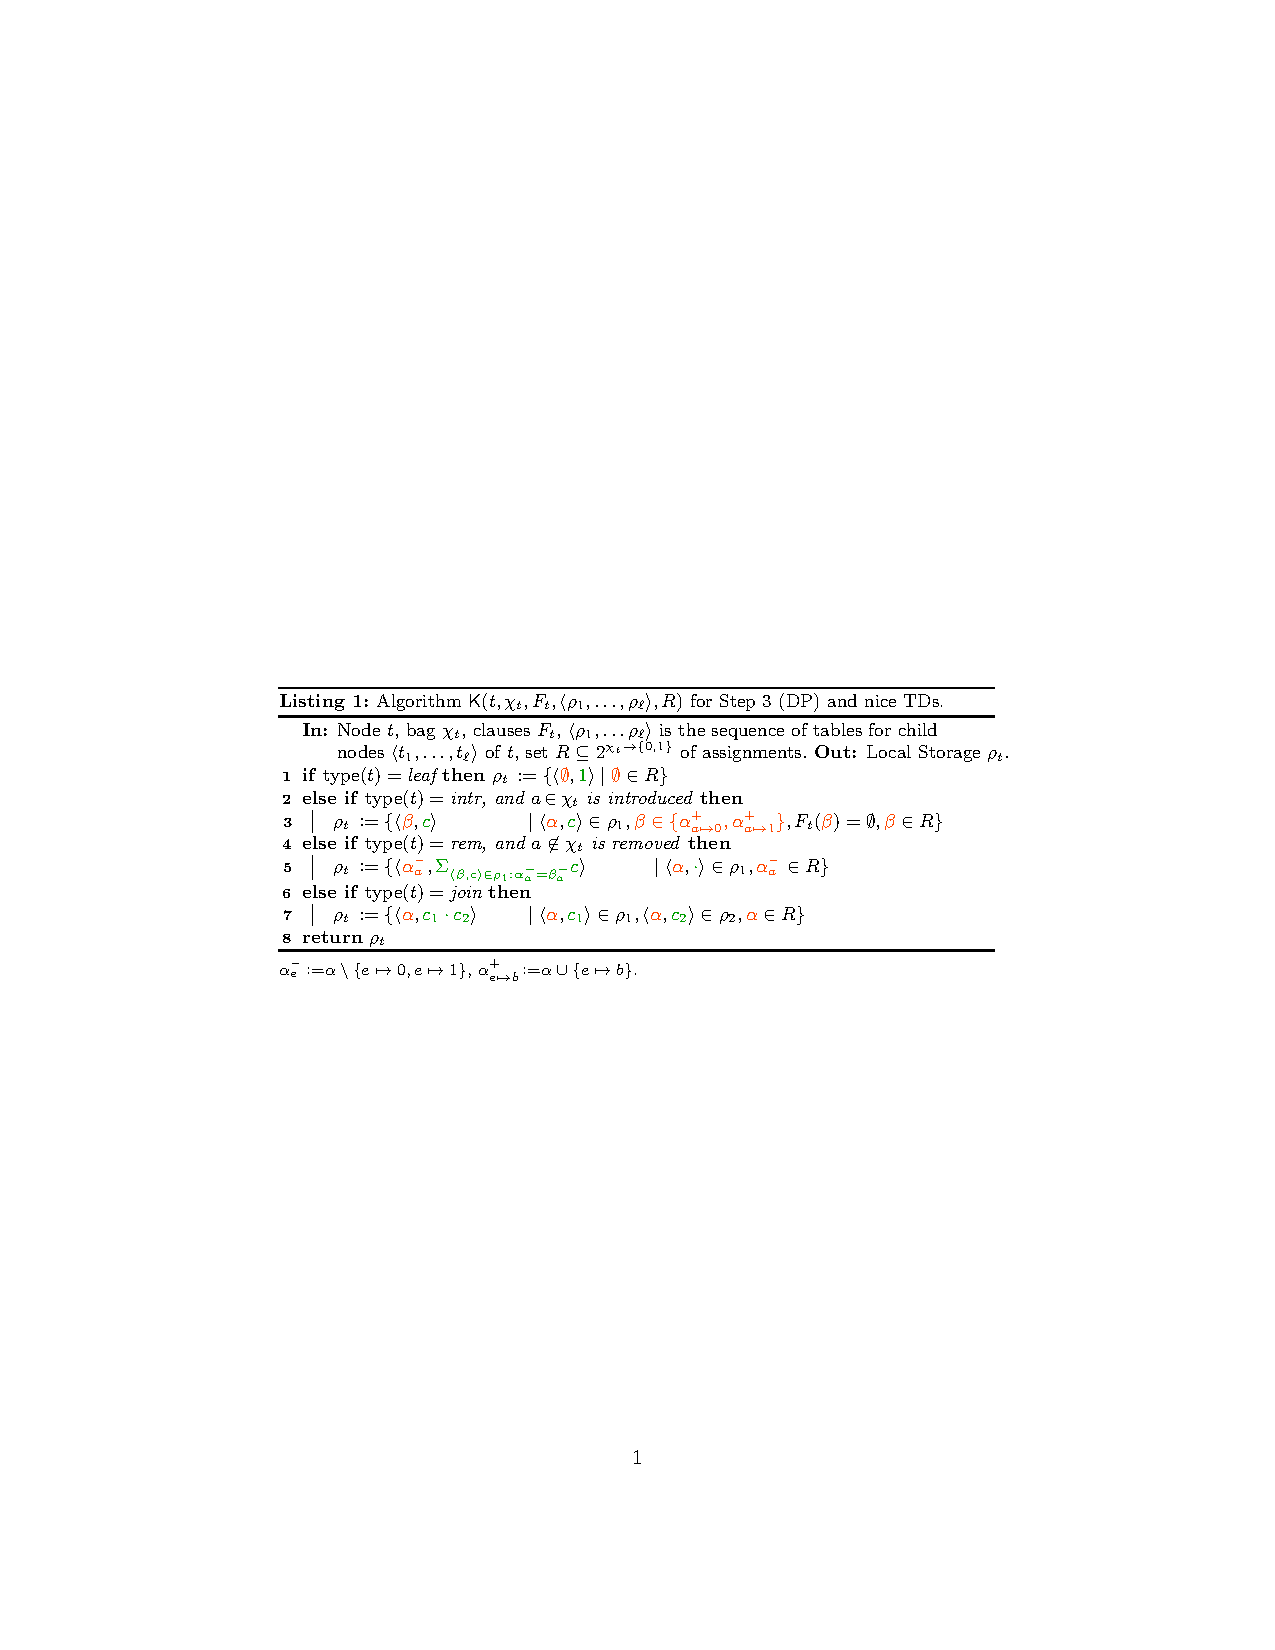
\includegraphics[trim={4.7cm 11.35cm 5cm 11.64cm},clip,page=1]{2-includes/prim.pdf}}
%
\end{figure*}


\paragraph*{Dynamic Programming on TDs.} %
%
%
A solver based on \emph{dynamic programming (DP)} for formulas
evaluates the input formula~$F$ in parts along a given TD of the
primal graph~$P_F$.  For each node~$t$ of the TD, results are usually
stored in a \emph{local storage}~$\rho_t$.
%
The approach works in four steps as follows:
\begin{enumerate}%
\item Construct the primal graph~$P_F$ of the input formula~$F$.
\item Heuristically compute a tree decomposition~$\TTT=(T,\chi)$ of
  the primal graph~$P_F$.
\item\label{step:dp} DP: Traverse the nodes in~$V(T)$ in
  post-order~$O$.\\
  At every node~$t \in O$, run an algorithm~$\algo{K}$ that takes as input %
  $t$, $\chi(t)$, the sub-formula~$F_t$ and previously computed results of its
  children and stores the results in~$\rho_t$, which in turn is used by the algorithm at
  the parent (if exists). 
\item Print the (weighted) model count by interpreting the
  result~$\rho_n$, which has been computed for the root~$n$ of~$T$.
\end{enumerate}

\noindent Algorithm~$\algo{K}$ in Step~\ref{step:dp} for nice TDs is depicted in Listing~\ref{fig:prim1}, cf.,~\cite{FichteEtAl18c,SamerSzeider10b}. Let therefore parameter~$R$ (``range'') of~\algo{K}
be a set of assignments, i.e., $R\subseteq 2^{\chi(t) \rightarrow \{0,1\}}$.
We assume~$R=2^{\chi(t) \rightarrow \{0,1\}}$ for sequential DP.
Then, algorithm~\algo{K} stores in~$\rho_t$ pairs of the form~$\langle\alpha,c\rangle$
consisting of an assignment~$\alpha: \chi(t) \rightarrow \{0,1\}$ together with a counter~$c$. %
Each pair~$\langle \alpha, c\rangle$ indicates that there are~$c$ many satisfying assignments restricted to~${\chi(t)}$ of~$F_{\leq t}$.
These pairs are carefully maintained for all the different types of nodes of nice TDs in Listing~1.
%
For details, we refer to the
literature~\cite{FichteEtAl18c,SamerSzeider10b}.
%
%

While in theory we often prefer nice TDs, due to simpler cases
distinctions, in an actual implementation of~\algo{K} one handles also
interleaved cases.  Note that a very compact way to represent~$\rho_t$
is simply by taking a sequence of model counts~$c$ for the
sub-formula~$F_{\leq t}$ without explicitly storing~$\alpha$ for a
fixed ordering of the considered assignments.
%
Each counter in the sequence is entirely independent of another
counter in the sequence as each counter in~$\rho_t$ depends only on
results previously computed at the children. This allows directly to
parallelize the computation of the counts in~$\rho_t$.
%
%
Since we have $2^{\Card{\chi(t)}}$ many assignments at each node~$t$, for
which we can compute the (potentially zero) counters by the very same
operations, we can immediately parallelize the operations on the
GPU~\cite{FichteEtAl18c} by employing a \emph{single instruction on
  multiple threads (SIMT)} computation model.
%
More detailed, $\algo{K}$ in Step~\ref{step:dp} refers
to a program that can be executed by a GPU thread, taking a small set
of instructions but multiple input data, e.g., different ranges~$R$.
Then, for each node~$t$ one can compute~$\rho_t$
for $\Card{2^{\chi(t)}}$ many (singular) ranges in parallel. 
Such a procedure is also
called \emph{(GPU-)kernel} for this hardware architecture.
%
The simplest possible data structure for~$\rho_t$ is an \emph{array} that just
contains the counts, where an assignment is addressed by the memory
address (index) of an entry in the array.
%
However, this data structure has to be allocated on the \emph{video
  RAM (VRAM)} prior to running the kernel on the GPU.
There, one has to take care of %
%
out-of-memory issues caused by huge space requirements.
%

\section{An Improved GPU-based DP Architecture}
%
In this section, we build upon the idea above and
present an innovative architecture for parallel
dynamic programming on the GPU, which is outlined in Figure~\ref{fig:gpudp}.
%
%
%
Novel parts of the architecture are the
\emph{preprocessors}, tree \emph{decomposition selection} heuristics
(customized TDs), generalization to allow for adaptable, more advanced
\emph{data structures}, \emph{caching} intermediate results on the
GPU, and the idea of \emph{compressing} counters for assignments.
%
%
%
%
Note that the architecture is independent from the underlying data
structures, i.e., in Step~\ref{step:dp} we refer by~$\rho_t$ to a
storage for data in the RAM, which can be an array or another data structure.
Analogously, $\iota_t$ also denotes a storage, that caches results in
the VRAM for GPU computations.  In the following, we discuss the novel
steps of the architecture, whereas details on data structures are
presented in Section~\ref{sec:implementation}.
%
%

\paragraph*{Step 0: Instance Preprocessing.}
Before we decompose our instance, we \emph{simplify the formula~$F$}
by a preprocessor for 
formulas~\cite{LagniezLoncaMarquis16a,LagniezMarquis14a}. There, we
preserve the number of satisfying assignments and potentially decrease
the treewidth of~$F$. For weighted model counting,
vivification and literal elimination can be
applied~\cite{LagniezMarquis14a}.

\begin{figure*}[t]
   \resizebox{1\columnwidth}{!}{%
     \includegraphics{1-figs/figure_gpu.pdf}
     %
   }
\centering
\caption{%
  Architecture of our DP-based solver for parallel execution. Yellow
  colored boxes indicate tasks that are required as initial step for
  the DP-run or to finally read the model count from the computed
  results.  The parts framed by a dashed box illustrate the DP-part.
  Boxes colored in red indicate computations that run on the
  CPU. Boxes colored in blue indicate computations that are executed
  on the GPU (with waiting~CPU).}
\label{fig:gpudp}
\end{figure*}

\paragraph*{Step 2: Tree Decomposition Computation.}
%
In Step~2.I, we heuristically compute a tree decomposition for the
dynamic programming.
%
Various recent literature
suggests~\cite{AbseherMusliuWoltran17b,CharwatWoltran17,JegouNdiayeTerrioux05}
that tree decompositions for practical solving require in addition to
``small'' width other criteria to speed up the performance of a
solver. Such tree decompositions are frequently called
\emph{customized tree decompositions}.
%
We compute $m$ different tree decompositions via
heuristics~\cite{AbseherMusliuWoltran17a} and then select among
the~$m$ decompositions one decomposition according to a selection criterion. In the
implementation, we use the library \emph{htd} version~1.2 with default
settings~\cite{AbseherMusliuWoltran17a} where $m = 30$. The selection
criterion is as follows. We first try to minimize the width. Then, if
several decompositions of the same width are found, we select the
decomposition with the smallest maximal cardinality~$v(\TTT)$ of the
intersection of bags of any node with its children, i.e.,
$v(\TTT)=\max\SB \Card{\chi_t \cap (\chi_{t_1} \cup \chi_{t_2} \cup
  \ldots \cup \chi_{t_\ell}) } \SM t \in V(T), t_1,t_2, \ldots, t_\ell
\text{ are children of } t \text{ in } T \SE$ where
$\TTT =(T, \chi)$.
%
The idea of the selection is to balance the \emph{trade-off} between
runtime and space requirements in the worst-case as outlined in
earlier work~\cite{JegouNdiayeTerrioux05}. In that way, we first
improve on the worst-case \emph{runtime (and VRAM consumption)} and
then on the number of IO operations required to copy data between RAM
and VRAM.
%
%
%
%
%
%
After the selection of tree decomposition~$\mathcal{T}$, we
\emph{preprocess~$\mathcal{T}$} (Step~2.II).  There, we combine nodes to
obtain bags of size~$s$, which is the largest number such that on the
chosen hardware~$2^s$ GPU threads can still run in parallel. This 
reduces the overhead of copying onto VRAM, and GPU
thread allocation.


\subsection*{Step \ref{step:dp}: Dynamic Programming
}
The more involved architecture of Step~\ref{step:dp} %
consists of multiple parts as follows.
%
%
%
%

\paragraph*{Step \ref{step:dp}.I: Search Space Partitioning.}
%
As described in the preliminaries, the DP proceeds by traversing a tree
decomposition in post-order. %
%
At each node, we consider assignments restricted to the variables in
$\chi(t)$ and its corresponding counters. Overall we can have at
most~$2^{\Card{\chi(t)}}$ assignments (``local search space'' at a
node). Thus, the number of assignments can simply be too large to even
store just one counter per assignment in the VRAM.
%
In practice, we would expect that plenty of these assignments result
in a counter that is zero and hence we could actually avoid the
out-of-memory issue as data can be compressed. However, on the VRAM we
have to allocate memory prior to the computation and hence it would
require to detect the point where we run out-of-memory then to copy the
data back to the RAM resulting in turn in an unutilized GPU.
%
To avoid this situation, we simply split in Step~\ref{step:dp}.I all
possible assignments that are considered together at once on the GPU
into several disjoint subsets~$S_1, S_2, \ldots, S_k$
of~$2^{\Card{\chi(t)}}$, which we call \emph{search space
  partitioning}.
%
%
%
%
On these grounds, we do the solution space splitting before the GPU kernels are
even executed to ensure that no out-of-memory issue occurs.
%
Splitting is independent of the actually used data structure and
can, e.g., be used if we store counters in an array similar to~\gpusatone.
%


\paragraph*{Step \ref{step:dp}.II: Splitting Input Result from Children
  and Compression.}
%
In the next step, we systematically process each set~$S_i$ for
$1 \leq i \leq k$. Therefore, we consider the assignments in~$S_i$ and
the corresponding counters for the children, i.e., the counters and
corresponding assignments at the children which we need to compute the
counter for an assignment at the currently considered node~$t$.
%
Since we have both to copy these relevant assignments of the children
onto the VRAM and still allocate enough VRAM for~$S_i$, we might
run into the situation that both would not fit into the VRAM.
%
Hence, we need to split for the counts and its corresponding
assignments in~$S_i$ the relevant results
in~$\rho_{t_1}, \ldots, \rho_{t_\ell}$ computed at the child
nodes~$t_1, \ldots, t_{\ell}$ of~$t$ into
subsets~$C_1\subseteq \rho_{t_1}$, $\ldots$,
$C_{\ell} \subseteq \rho_{t_\ell}$.  We call a
tuple~$\vec C=\langle C_1$, $\ldots$, $C_\ell\rangle$ of these subsets
\emph{chunk}.  Then, the \emph{chunk handler} systematically takes
each tuple~$\vec C$ relevant for~$S_i$ and executes a kernel in a GPU
thread for each element in~$S_i$ using~$\vec C$.
%
Subsequently, the resulting counts are summed up accordingly and kept
inside cache storage~$\iota_t$ on the VRAM.
%
This allows to reduce the number of IO operations between RAM and VRAM
for tree decompositions of larger width.
%
Finally, if all chunks are processed for~$S_i$, the memory
region~$\iota_t$ is merged into the RAM~$\rho_t$ for node~$t$.
%
There, depending on the data structure, it can be beneficial to merge
and \emph{compress} resulting solutions obtained for two different
solution spaces~$S_i$ and $S_j$.
For this task, we use a \emph{(support) kernel} on the GPU,
where one can merge two regions, say $\iota^{(i)}_t$ and $\iota^{(j)}_t$,
into memory~$\rho_t$, with the same idea for parallelization as in~\algo{K},
in parallel. In turn, this
might decrease the number of child chunks needed at the parent of~$t$.
%
%
%
In other words, for the parent node of~$t$,
one might prevent splitting results~from~children.

\section{Data Representation}
\label{sec:implementation}
%
We implemented our
solver~\gpusatnu{} %
based on the architecture presented in the previous section.
%
In this section, we describe advancements in the implementation of the
solver such as \emph{data structures} optimized for GPUs, and improved
accuracy in form of \emph{log-counters}.
%
%

\subsection{Binary Search Tree on the GPU}
A naive approach to store counters on the VRAM~$\iota_t$ is simply to
exhaustively consider all possible assignments in $2^{\chi(t)}$ and
store for each assignment a counter, even if zero, in an array.
%
%
In order to compactly store assignments at a node~$t$ in the VRAM, we
propose a new data structure, which is in a broader sense a
\emph{binary search tree (BST)} for assignments on a very low level
architecture.
%
The binary search tree contains only assignments to~$F_t$ whose
corresponding counter is non-zero, i.e., only counters for
assignments that can be extended\footnote{Extending an assignment can be
  done by recursively considering previously computed assignments at
  the children that correspond to an assignment at the node.} to
satisfying assignments of~$F_{\leq t}$.
%
%
The BST data structure allows us to allocate memory on the VRAM in
advance, which is required by~OpenCL~1.2, as kernels itself are not
allowed to allocate memory on the VRAM during the execution.
%
Further, it allows us to avoid of synchronization between threads.
%

%
Internally, a BST consists of a continuous sequence of \emph{cells}
that are implemented as 64-bit unsigned integers.  We have three types
of cells, namely \emph{empty cells}, \emph{value cells}, and
\emph{index cells}.  An empty cell contains a zero whereas a value
cell contains an integer greater than zero.  For value cells the
64-bit integer corresponds to a counter that is internally actually
interpreted as a double floating point type. We discuss details in the
next paragraph.
%
Index cells have either one or two successors in the tree and refer to
a value or index cell.
 %
For an index cell, the \emph{lower 32 bits} of the integer represent the
\emph{index} to the next cell, where a corresponding variable is set to
false.  Symmetrically, the \emph{upper 32 bits} form an index to the cell if
the variable is set to true.  Note that either the lower or upper bits
can be zero indicating that the respective index is empty.
%
In Example~\ref{ex:bst} we illustrate BST memory allocation including
the three types of cells by a simple example where an assignment is
inserted into a non-empty previously BST.


\begin{figure}[t]
  \centering %
  %
  %
  %
  %
  %
  %
  %
  %
  %
  %
  %
  %
  %
  %
  %
  %
  %
  \resizebox{0.3\textwidth}{!}{
    \setlength\tabcolsep{0.5em}
    \begin{tabular}{{c|c||cc}}
      \toprule
      \multirow{2}{*}{(index)} & \multirow{2}{*}{(var)} & \multicolumn{2}{c}{cell}\\
                               & & low & high \\
      \midrule
      0 & $x$ & $\epsilon$ & 1\\
      1 & $y$ & 3 & 2\\
      %
      2 & - & \multicolumn{2}{c}{\textbf{23}}\\
      3 & - & \multicolumn{2}{c}{\textbf{42}}\\
      4 & & \multicolumn{2}{c}{$\epsilon$}\\
      $\ldots$ & $\ldots$ & \multicolumn{2}{c}{$\ldots$}\\
      &&\\
      &&\\
    \end{tabular}
  }
  \hspace{4em}
  %
  \resizebox{0.3\textwidth}{!}{
    \setlength\tabcolsep{0.5em}
    \begin{tabular}{{c|c||cc}}
      \toprule
      \multirow{2}{*}{(index)} & \multirow{2}{*}{(var)} & \multicolumn{2}{c}{cell}\\
                               & & low & high \\
      \midrule
      0 & $x$ & 4 & 1\\
      1 & $y$ & 3 & 2\\
      %
      2 & - & \multicolumn{2}{c}{\textbf{23}}\\
      3 & - & \multicolumn{2}{c}{\textbf{42}}\\
      4 & $y$ & $\epsilon$ & 5\\
      5 & - & \multicolumn{2}{c}{\textbf{1}}\\
      6 & & \multicolumn{2}{c}{$\epsilon$}\\
      $\ldots$ & $\ldots$ & \multicolumn{2}{c}{$\ldots$}
    \end{tabular}
    %
  }%
\caption{Initial BST~$\mathcal{B}$ (left) and BST~$\mathcal{B}'$ (right),
which was obtained after inserting assignment $\{x\mapsto0, y\mapsto1\}$.
Value cells are depicted in bold. Both empty cells and empty indices are
indicated by the symbol~$\epsilon$. Note: We store \emph{only} cells (``low'', ``high'').}
\label{fig:treeexample}
\end{figure}


%
%
%
%
%
%
%
%
%
%
%
%
%
%
%
%
%
%
%
%
%
%
%
%
%
%
%
%
%
%
%
%
%
%
%
%
%
%
%
%
%
%
%
%
%
%
%
%
%

%

\begin{example}\label{ex:bst}
  Figure~\ref{fig:treeexample} (left) illustrates a binary search
  tree~$\mathcal{B}$, where value cells are depicted in \textbf{bold}
  face. Both empty cells and empty indices are represented by the
  symbol~``$\epsilon$''.
%
  %
  %
  In the
  BST~$\mathcal{B}$ we assume $x<y$.
 %
  In Figure~\ref{fig:treeexample} (right), we can see the
  BST~$\mathcal{B}'$ obtained by inserting the
  assignment~$\alpha\eqdef\{x\mapsto0, y\mapsto1\}$
  into~$\mathcal{B}$.
%
  %
%
  In order to insert~$\alpha$, we recursively search for~$\alpha$ in~$\mathcal{B}$
  by traversing~$\mathcal{B}$ according to the variable order,
  beginning at start index~$0$.  Then, depending on the assignment of
  the variable at index~$0$ in~$\alpha$, we continue searching using
  the next variable at the respective index.
%
%
  As soon as an empty index is found, %
  %
  new index cells for the remaining variables are
  subsequently inserted, followed by an inserted value cell of
  value~\textbf{1}.  As a result, the search for~$\alpha$
  in~$\mathcal{B}$ stops at the lower 32 bits of the index cell at
  index~$0$. In turn, these bits refer to a new index cell
  for~$y$ at index~$4$, whose upper 32 bits point to a new value
  cell at index~$5$.
\end{example}
%
%
Note that we need some \emph{fixed order on the variables}
in~$\chi(t)$, to distinguish index and value cells in order to
search, insert, update, and delete counters for a given assignment
over the variables.
%
The binary search tree enables us to address~$2^{32}-1$ many 64-bit
integers, which can be changed to relative indices (offsets) if more
address space is required.
%
%
%
%
Further, for a given number~$b$ of
variables, the tree requires in the worst-case at most~$2^{b+1}-1$
many 64-bit integers, since there are at most~$2^b$ many value cells
(all assignments have non-zero counters) and~$2^b-1$ index cells
(perfectly balanced BST) needed.
%
%

Obviously, our data structure has to be manipulated by several GPU
threads in parallel.  In contrast to the array data structure, where
each GPU thread has unique access to one entry, the BST has to
\emph{prevent race conditions} between threads.  Our strategy is
to allow atomic write access only to non-empty cells.
To this end, we keep track of the number of non-empty cells of the tree, and 
assign indices of non-empty cells in ascending order. 
Then, we need (i) to atomically reserve free (empty) indices and (ii) to run only synchronized updates on existing value cells.
%
In the actual implementation this is efficiently done by \emph{atomic
  operations} for 32-bit and 64-bit data types provided by the OpenCL
framework~\cite{MunshiGasterMattson11a}.
%
In Case~(i) we rely on \ops{atomic\_cmpxchg} for inserting into the index, but only if it is empty (atomic operation).
In Case~(ii) we use \ops{atomic\_add} for concurrently~updating~counters.

\paragraph{Balancing between BST and Arrays.}
It is easy to see that the BST data structure introduces an overhead
in the computation. For instances of small width where all
possible partial truth assignments (and the counts even if 0) easily
fit into the VRAM using an array, the BST might not pay off.
%
Hence, one can also design an implementation that uses the array up to
a threshold and then switches to BST as a data structure. We
implemented this option into our solver and call the resulting variant
\gpusatnuv{A+B}.
Further, whenever \gpusatnu{} has to combine BSTs %
for a node with more than one child node, we use a support kernel
for transforming BSTs into arrays. Kernel~\algo{K} then combines the arrays into a BST.
%
%



%
%
%
%
%
%
%
%
%
%
%
%
%
%
%
%
%


\subsection{Accuracy of Large-Scale Counters}
In order to be able to apply our solver to instances with very high
solution count while still preserving a high accuracy, we store the
model count during the dynamic programming by the log of the value.
%
This technique is common in the domain of probabilistic inference and
also known as \emph{log-counter}.


In more detail, we described in the previous paragraph that one could
take 64-bit floating point numbers to store the values of a
counters. While IEEE 64-bit floating point numbers allow to represent
only values below~$10^{308}$~\cite{ieee754}, counters can have a
significantly higher value.
%
Therefore, we need an extended data type for each counter~$c$. We
store the value of~$c$ in relation to~$2^{e}$ for a 64-bit integer~$e$.
%
%
%
We start with significant digit~$1$ before the decimal point where
$c=1.x \cdot 2^e$ and chosen $e$ accordingly. Then, we store $1.x$ and
$e$ to reconstruct the value of~$c$.
%
In the implementation, we start with $e = 0$ and increase it
dynamically during the computation at a node~$t$ whenever
necessary. We normalize the largest counter~$c$ at a node~$t$ as
decribed above and all other counters computed at node~$t$ are
represented with the same exponent~$e$, i.e., we need only one
exponent per node. We call the resulting $e$ the \emph{largest
  exponent for~$t$}.
%
In that way, we remain highest accuracy while still being
able to represent high values.
%
The largest exponent is carefully maintained on the GPU during
computation of~$\rho_t$ in kernel~$\algo{K}$ and passed along to
parent nodes.
%
For the largest exponents at a node, which has more than one child
(join node), we may have to combine counters with respect to different
largest exponents for child nodes of~$t$.
In more details, algorithm~\algo{K} additionally takes the sum~$e$ of the largest %
exponents~$e_1$, $e_2$, $\ldots$ of its children as parameter,
which represent the counters. %
%
Exponent~$e$ is then also used to represent counters at~$t$, however,
it might increase during the computation and therefore~\algo{K}
returns an updated exponent after the computation.

%

\section{Experiments}
\label{sec:experiments}
%
We conducted a series of experiments using several benchmark sets for
model counting and weighted model counting. Benchmark
sets~\cite{FichteEtAl18b} and our results~\cite{FichteEtAl19c} are
publicly available and also on github at
\href{https://github.com/daajoe/gpusat_experiments/tree/cp2019}{\nolinkurl{daajoe/gpusat_experiments}}.



\paragraph{Measure, Setup, and Resource Enforcements.}
As we use different types of hardware in our experiments and other
natural measures such as power consumption cannot be recorded with
current hardware, we compare wall clock time and number of
timeouts. In the time we include, if applicable, \emph{preprocessing
  time} as well as \emph{decomposition time} for computing 30
decompositions with a random seed and decomposition selection time.
%
However, we avoid IO access on the CPU solvers whenever possible,
i.e., we load instances into the RAM before we start solving.
%
For parallel CPU solvers we allow access to 12 or 24 physical cores on
machines where hyperthreading was disabled.
%
%
%
%
%
We set a timeout of 900 seconds and limited available RAM to~14 GB per
instance and solver.

\paragraph{Benchmark Instances.}
We considered a selection of overall 1494 instances from various
publicly available benchmark sets for model counting consisting of %
%
%
%
%
\instances{fre/meel} benchmarks\footnote{See:
  \href{http://tinyurl.com/countingbenchmarks}{\nolinkurl{tinyurl.com/countingbenchmarks}}}(1480
instances), %
and \instances{c2d} benchmarks\footnote{See:
  \href{http://reasoning.cs.ucla.edu/c2d/results.html}{\nolinkurl{reasoning.cs.ucla.edu/c2d}}}
(14 instances).
%
For~\WMC, we used the overall 1091 instances from the
\instances{Cachet} benchmark set\footnote{See:
  \href{https://www.cs.rochester.edu/u/kautz/Cachet/Model_Counting_Benchmarks/index.html}{\nolinkurl{cs.rochester.edu/u/kautz/Cachet}}}.
%

\paragraph{Benchmarked Solvers.}
In our experimental work, we present results for the most recent
versions of publicly available \cSAT solvers, namely,
%
\href{http://reasoning.cs.ucla.edu/c2d/download.php}{\textit{c2d}~2.20}~\cite{Darwiche04a},
\href{http://www.cril.univ-artois.fr/KC/d4.html}{\textit{d4}~1.0}~\cite{LagniezMarquis17a},
\href{https://bitbucket.org/haz/dsharp}{\textit{DSHARP}~1.0}~\cite{MuiseEtAl12a},
\href{http://reasoning.cs.ucla.edu/minic2d/}{\textit{miniC2D}~1.0.0}~\cite{OztokDarwiche15a},
\href{http://www.cril.univ-artois.fr/KC/eadt.html}{\textit{cnf2eadt}~1.0}~\cite{KoricheLagniezMarquisThomas13a}, 
\href{http://www.sd.is.uec.ac.jp/toda/code/cnf2obdd.html}{\textit{bdd\_{}minisat\_\allowbreak{}all}~1.0.2}~\cite{TodaSoh15a},
and \href{http://reasoning.cs.ucla.edu/sdd/}{\textit{sdd}~2.0}~\cite{Darwiche11a} (based on %
knowledge compilation techniques).
%
%
%
%
%
%
%
We also considered rather recent approximate solvers
\href{https://bitbucket.org/kuldeepmeel/approxmc}{\textit{ApproxMC2}, \textit{ApproxMC3}}~\cite{ChakrabortyEtAl14a}
and
\href{http://cs.stanford.edu/~ermon/code/STS.zip}{\textit{sts}~1.0}~\cite{ErmonGomesSelman12a},
%
as well as %
CDCL-based solvers
%
\href{https://www.cs.rochester.edu/u/kautz/Cachet/cachet-wmc-1-21.zip}{\textit{Cachet}~1.21}~\cite{SangEtAl04},
\href{http://tools.computational-logic.org/content/sharpCDCL.php}{\textit{sharpCDCL}}\footnote{See:
  \href{http://tools.computational-logic.
    org/content/sharpCDCL.php}{\nolinkurl{tools.computational-logic.
      org}}}, %
and
\href{https://sites.google.com/site/marcthurley/sharpsat}{\textit{sharpSAT}~13.02}~\cite{Thurley06a}.
%
Finally, we also included multi-core solvers
\href{https://github.com/daajoe/GPUSAT/releases/tag/v0.815-pre}{\textit{gpusat}~1.0}~\cite{FichteEtAl18c}, as well as
\textit{countAntom}~1.0~\cite{BurchardSchubertBecker15a} on 12 physical CPU
cores, which performed better than on 24 cores.
%
%
%
%
%
%
%
%
Note that we benchmarked additional solvers, which we omitted from the
presentation here and where we placed results online in our result
data repository.
%
For~\WMC, we considered the following solvers: \textit{sts},
\textit{\gpusatone}, \gpusatnu, \textit{miniC2D}, \textit{Cachet},
\textit{d4}, and
\href{http://www.cril.univ-artois.fr/kc/ressources/query-dnnf-0.4.180625.zip}{\textit{d-DNNF
    reasoner}~0.4.180625} (on top of d4 as underlying knowledge
compiler). %
All experiments were conducted with default solver options.
%
%
For solver~\gpusatnu, we also benchmarked variant~\gpusatnuv{A+B}
where we used 30 as threshold above which we apply the BST.
%
%
%
%
%
%
%



\begin{figure}[bt]
\centering
\vspace{0pt}\includegraphics[height=13em]{plot_Width_sat.pdf}%
\hspace{6pt}\includegraphics[height=13em]{plot_Width_wmc.pdf}%
\caption{%
  Width distribution of~\cSAT instances (left) before and after
  preprocessing (using both B+E and pmc).  Width distribution of~\WMC
  instances (right) before and after preprocessing using pmc*.
  Results are based on the primal treewidth and presented in
  intervals.  X-axis labels the intervals, y-axis labels the number of
  instances.
%
}%
\label{fig:distribution}
\end{figure}
%

\paragraph{Benchmark Machines.}
%
%
%
%
The non-GPU solvers were executed on a cluster of 9 nodes. Each node is equipped
with two Intel Xeon E5-2650 CPUs consisting of 12 physical cores each
at 2.2 GHz clock speed and 256 GB RAM. %
The results were gathered on Ubuntu~16.04.1 LTS machines with disabled hyperthreading
on kernel~4.4.0-139, which is already a post-Spectre and
post-Meltdown kernel\footnote{Details on spectre and meltdown: \href{https://spectreattack.com/}{\nolinkurl{spectreattack.com}}.}.
%
%
For~\gpusatone and~\gpusatnu we used a machine equipped with a consumer GPU:
%
Intel Core i3-3245 CPU operating at 3.4 GHz, 16 GB RAM, and one
Sapphire Pulse ITX Radeon RX 570 GPU running at 1.24 GHz with 32
compute units, 2048 shader units, and 4GB VRAM using driver
amdgpu-pro-18.30-641594 and OpenCL~1.2.
The system operated on Ubuntu~18.04.1 LTS with kernel 4.15.0-34.
%




%
%
%
%
%
%
%
%
%
%
%
%
%
%
%
%
%
%
%
%
%
%
%
%
%
%
%
%
%
%
%
%
%
%
%



\begin{table}[bt]
  \centering
  \resizebox{\columnwidth}{!}{%
    \begin{tabular}{{l|l|rr|rHr|rHr||rrrrr||rrrH}}
      \toprule
      prob & pre &  vMdn & cMdn & t[s] Mdn & t[s] Max & to & t[s] Mdn pre & t[s] Max pre & to & Mdn & 50\% & 80\% & 90\% & 95\% & min & max & mdn & mean \\
      \midrule
      \cSAT & w/o pre & 637 & 810 & 0.07 & 1800.0 & \textbf{6} & n/a & n/a & n/a & 31 & 31 & 166 & 378 & 922 & n/a & n/a & n/a & n/a \\
      & pmc, B+E & \textbf{231} & 350 & 0.02 & 1800.0 & \textbf{6} & 0.06 & 900.0 & 192 & \textbf{3} & \textbf{3} & \textbf{17} & 201 & \textbf{823} & -72 & \textbf{755} & 22 & \textbf{31.9} \\
      & pmc & \textbf{231} & 189 & 0.03 & 1800.0 & \textbf{6} & \textbf{0.03} & 900.0 & \textbf{103} & \textbf{3} & 4 & 19 & 228 & \textbf{823} & -1839 & 547 & \textbf{23} & 23.1 \\
      & B+E & \textbf{231} & \textbf{185} & \textbf{0.02} & 1800.0 & \textbf{6} & 0.04 & 900.0 & 189 & \textbf{3} & \textbf{3} & 18 & \textbf{192} & \textbf{823} & 
                                                                                                                                                                    \textbf{-2} & 633 & \textbf{23} & 31.7 \\
      \midrule
      \WMC & w/o pre & \textbf{200} & 519 & 0.04 & 9.21 & \textbf{0} & n/a & n/a & n/a & 28 & 28 & 40 & 43 & 54 & n/a & n/a & n/a & n/a \\
           & pmc* & \textbf{200} & \textbf{300} & \textbf{0.03} & 1.6 & \textbf{0} & \textbf{0.03} & 1.6 & \textbf{0} & \textbf{11} & \textbf{11} & \textbf{20} & \textbf{25} & \textbf{30} & \textbf{0} & \textbf{330} & \textbf{16} & \textbf{18.8} \\
      \bottomrule
    \end{tabular}
  }
  \medskip
  \caption{Overview on upper bounds of the primal treewidth for
    considered \cSAT and \WMC benchmarks before and after
    preprocessing.  vMdn median of variables, cMdn median of clauses,
    t[s] Mdn of the decomposition runtime in seconds, maximum runtime
    t[s] Max, median Mdn and percentiles of upper bounds on treewidth,
    and min/max/mdn %
    of the width improvement after preprocessing. Negative values
    indicate worse results.  }
\label{tab:tw_combined}
  \label{tab:tw_combined_wmc}
\label{tab:detailed}
\end{table}

\subsection{Results}
First, we present how existing preprocessors for \cSAT and
equivalence-preserving preprocessors for~\WMC influence the treewidth
on the considered instances.






\paragraph{Treewidth Analysis.}
We computed upper bounds on the primal %
treewidth for our benchmarks before and after preprocessing and state
them in intervals.
%
For model-count preserving preprocessing we
explored both
\href{http://www.cril.univ-artois.fr/kc/bpe2.html}{B+E~Apr2016}~\cite{LagniezLoncaMarquis16a}
and
\href{http://www.cril.univ-artois.fr/kc/pmc.html}{pmc~1.1}~\cite{LagniezMarquis14a}.
%
For \WMC, we used pmc with documented options \ops{-vivification}
\ops{-eliminateLit} \ops{-litImplied} \ops{-iterate=10} to preserve
all the models, which we refer to by~\emph{pmc*}.
%
%
In this experiment, we used different timeouts. We set the timeout of
the preprocessors to 900 seconds and allowed further 1800 seconds for
the decomposer to get a detailed picture of treewidth upper bounds.
%
Figure~\ref{fig:distribution} (left) presents the width distribution
of number of instances (y-axis) and their corresponding upper bounds
(x-axis) for primal treewidth, both before and after preprocessing
using B+E, pmc, and both preprocessors in combination (first pmc, then
B+E) for~\cSAT.
%
Table~\ref{tab:tw_combined} (top) provides statistics on the
benchmarks combined, including runtime of the preprocessor, runtime of
the decomposer to obtain a decomposition, upper bounds on primal
treewidth, and its improvements before and after
preprocessing. 
%
Further, the table also lists the median of the widths of the obtained
decompositions and their percentiles, which is the treewidth upper
bound a given percentage of the instances have.
%
%
%
Interestingly, overall we have that a majority of the instances
after preprocessing has width below~20.
%
In more details, more than 80\% of the \cSAT instances have primal 
treewidth below~19
after preprocessing, whereas 90\% of the instances have
treewidth below~192 for B+E.
%
With pmc we observed a corner case where the primal treewidth upper
bound increased by 1839, however, on average we observed a mean
improvement on the upper bound of slightly above 23. %
The best improvement among the widths of all our instances was
achieved with the combination of pmc and B+E where we improved the
width by~755.
%
Overall, both B+E and pmc managed to \emph{drastically reduce} the
widths, the decomposer ran below 0.1 seconds in median.
%
Interestingly, even the upper bounds on the treewidth of the \WMC
instances reduced with pmc* as depicted in
Figure~\ref{fig:distribution} (right).  In more detail, after
preprocessing 95\% of the instances have primal treewidth below~30,
c.f., Table~\ref{tab:tw_combined} (bottom).
%


\paragraph{Solving Performance Analysis.}
%
%
%
%
%
%
%
%
%
%


\begin{figure}[t]
  %
  %
  \centering
  \resizebox{.7\columnwidth}{!}{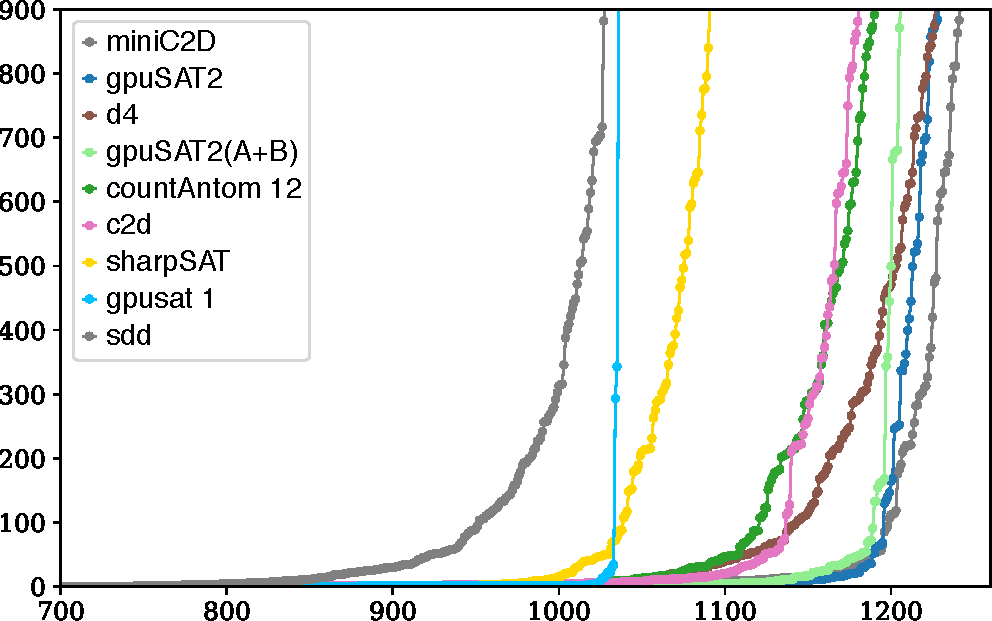
\includegraphics{plot_pmc_enlarged.pdf}}
  %
  %
  %
  %
  %
  %
  \caption{Runtime for the top 5 sequential and all parallel solvers over all the~\cSAT instances with pmc preprocessor. %
    %
    %
    The x-axis refers to the number of instances and the y-axis
    depicts the runtime sorted in ascending order for each solver
    individually.  }
  \label{fig:runtime}
\end{figure}
%
Figure~\ref{fig:runtime} illustrates the top five sequential solvers,
and all parallel counting solvers %
%
with preprocessor pmc %
%
in a cactus-like plot. 
Table~\ref{tab:sat:merged} presents detailed runtime
results for~\cSAT with preprocessors pmc, B+E, and without preprocessing, respectively.
%
%
%
%
%
%
%
%
%
%
%
%
%
%
%
%
Since the solver sts produced results that varied from the correct
result on average more than the value of the correct result, %
%
%
%
%
%
we excluded it from the presented results.  If we disallow
preprocessing, \gpusatnu and \gpusatone perform only slightly better
in the overall standing of the solvers. But \gpusatnu solves 42
instances more and requires about 10 hours less of wallclock
time. Further, we can observe, that %
the variant~\gpusatnuv{A+B} performs particular well, mainly since for
instances below width~30, the BST compression seems relatively
expensive compared to the array data structure.
%
%
%
%
%
Interestingly, when considering the results on preprocessing in
Table~\ref{tab:sat:merged} (top, mid) and Figure~\ref{fig:runtime} we
observe that the architectural improvements pay off quite
well. \gpusatnu can solve the vast majority of the instances and
ranks second place.  If one uses the B+E preprocessor shown in
Table~\ref{tab:sat:merged} (mid), \gpusatnu solves even more instances
as well as the other solvers. Still, it ranks fifth solving only 26
instances less than the best solver and 10 less than the third best
solver and solves the most instances having width below 30.

\newcommand{\inacc}[1]{\ensuremath{\diamond{}}#1}
\begin{table}[tb]
  \centering
  \resizebox{0.8\columnwidth}{!}{%
    \begin{tabular}{{l|lH||rrrrrrrr||r||rHr}}
      \toprule
      & solver & racc & 0-20 & 21-30 & 31-40 & 41-50 & 51-60 & $>$60 & best & unique & $\sum$ & time[h] & rank \\
      \midrule
      \parbox[t]{1em}{\multirow{9}{*}{\rotatebox[origin=c]{90}{pmc preprocessing}}}&miniC2D & \textbf{0} & 1193 & 29 & \textbf{10} & 2 & 1 & 7 & 13 & 0 & \textbf{1242} & \textbf{68.77} & 1 \\
      &\gpusatnu & 4.7E-15 & \textbf{1196} & 32 & 1 & 0 & 0 & 0 & 250 & %
                                                                                     \textbf{8} & 1229 & 71.27 & 2 \\
     %
      &d4 & \textbf{0} & 1163 & 20 & \textbf{10} & 2 & \textbf{4} & 28 & 52 & 1 & 1227 & 76.86 & 3 \\
      %
      & \gpusatnuv{A+B} & {4.6E-15} & {1187} & 18 & 1 & 0 & 0 & 0 & 120 & 7 & 1206 & 74.56 & 4 \\
      &countAntom 12 & \textbf{0} & 1141 & 18 & \textbf{10} & \textbf{5} & \textbf{4} & 13 & 101 & 0 & 1191 & 84.39 & 5 \\
      &c2d & \textbf{0} & 1124 & 31 & \textbf{10} & 3 & 3 & 10 & 20 & 0 & 1181 & 84.41 & 6 \\
      &sharpSAT & \textbf{0} & 1029 & 16 & \textbf{10} & 2 & \textbf{4} & \textbf{30} & \textbf{253} & 1 & 1091 & 106.88 & 7 \\
      &\gpusatone & 1.7E-13 & 1020 & 16 & 0 & 0 & 0 & 0 & 106 & 7 & 1036 & 114.86 & 8 \\
      & sdd & \textbf{0} & 1014 & 4 & 7 & 1 & 0 & 2 & 0 & 0 & 1028 & 124.23 & 9 \\
      %
      %
      \midrule
      & solver & racc & 0-20 & 21-30 & 31-40 & 41-50 & 51-60 & $>$60 & best & unique & $\sum$ & time[h] & rank \\
      \midrule
      \parbox[t]{1em}{\multirow{8}{*}{\rotatebox[origin=c]{90}{B+E preprocessing}}}&c2d & \textbf{0} & 1199 & 24 & \textbf{9} & 0 & 2 & 23 & 14 & 0 & \textbf{1257} & \textbf{63.46} & 1 \\
      &miniC2D & \textbf{0} & 1203 & \textbf{27} & 8 & 0 & 2 & 12 & 8 & 0 & 1252 & 64.92 & 2 \\
      &d4 & \textbf{0} & 1182 & 15 & \textbf{9} & \textbf{1} & \textbf{3} & 31 & 79 & 1 & 1241 & 69.32 & 3 \\
      &countAntom 12 & \textbf{0} & 1177 & 14 & 8 & 0 & 2 & \textbf{34} & 100 & 0 & 1235 & 69.79 & 4 \\
      %
      &\gpusatnu & 6.4E-16 & \textbf{1204} & 26 & 1 & 0 & 0 & 0 & \textbf{150} & \textbf{3} & 1231 & 68.15 & 5 \\
      %
      &\gpusatnuv{A+B} & {6.4E-16} & 1201 & 21 & 1 & 0 & 0 & 0 & 67 & \textbf{3} & 1223 & 70.39 & 6 \\
      &sdd & \textbf{0} & 1106 & 11 & 4 & \textbf{1} & 1 & 4 & 0 & 0 & 1127 & 100.48 & 7 \\
      &\gpusatone & 9.9E-12 & 1037 & 16 & 0 & 0 & 0 & 0 & 87 & %
                                                               \textbf{3} & 1053 & 110.87 & 8 \\
                                                               %
      &bdd\_minisat\_all & \textbf{0} & 926 & 6 & 3 & \textbf{1} & 1 & 0 & 101 & 0 & 937 & 140.59 & 9 \\
      %
      \midrule
      &solver & racc & 0-20 & 21-30 & 31-40 & 41-50 & 51-60 & $>$60 & best & unique & $\sum$ & time[h] & rank \\
      %
      \midrule
      \parbox[t]{1em}{\multirow{9}{*}{\rotatebox[origin=c]{90}{without preprocessing}}}& countAntom 12 & \textbf{0} & 118 & 511 & 139 & \textbf{175} & \textbf{21} & \textbf{181} & 318 & 15 & \textbf{1145} & \textbf{96.64} & 1 \\
      & d4 & \textbf{0} & 124 & 514 & 148 & 162 & \textbf{21} & 168 & 69 & 15 & 1137 & 104.94 & 2 \\
      & c2d & \textbf{0} & 119 & 525 & \textbf{165} & 161 & 18 & 120 & 48 & 15 & 1108 & 110.53 & 3 \\
      & miniC2D & \textbf{0} & 122 & 514 & 128 & 149 & 9 & 62 & 0 & 0 & 984 & 141.22 & 4 \\
      & sharpSAT & \textbf{0} & 100 & 467 & 124 & 156 & 12 & 123 & \textbf{390} & 4 & 982 & 135.41 & 5 \\
      %
      %
      %
      & \gpusatnuv{A+B} & {9.8E-18} & \textbf{125} & \textbf{539} & 96 & 138 & 0 & 0 & 94 
                                                                            & \textbf{19} & 898 & 151.16 & 8 \\
      %
                                                                            %
                                                                            %
                                                                            %
                                                                            %
                                                                            %
      &\gpusatnu & 9.7E-18 & \textbf{125} & 523 & 96 & 138 & 0 & 0 & 78 & 17 & 882 & 155.43 & 8 \\
      %
      &\gpusatone & 1.4E-10 & \textbf{125} & 524 & 67 & 140 & 0 & 0 & 82 & %
                                                                           9 & 856 & 162.03 & 11 \\
      &cachet & \textbf{0} & 99 & 430 & 71 & 152 & 8 & 57 & 3 & 0 & 817 & 176.26 & 12 \\
      %
      \midrule
      &solver & racc & 0-20 & 21-30 & 31-40 & 41-50 & 51-60 & $>$60 & best & unique & $\sum$ & time[h] & rank \\
      \bottomrule
    \end{tabular}
  }
  \caption{%
    Number of~\cSAT instances (grouped by treewidth upper bound intervals)
    solved by sum of the top five sequential and all parallel counting solvers 
    with preprocessor pmc (top), B+E (mid), and without preprocessing (bottom).
    time[h] is the cumulated  wall clock time in hours, where unsolved instances 
    are counted as 900 seconds.
%
  }%
  \label{tab:sat:merged}
%
\end{table}%

While we focus on \cSAT with our implementation, we also conducted the
experiments with \WMC in order to compare our solver with \gpusatone
in the setting for which it was designed.  Table~\ref{tab:wmcresults}
(top) lists results of the top five best solvers capable of
solving~\WMC on our instances. Compared to \gpusatone, our solver
\gpusatnu shows an improvement when the width of the instance is
between 21 and 40, in more detail \gpusatnu solves 44 instances more.
%
%
%
%
%
%
After preprocessing with~pmc*, one can observe that the majority of
the instances has width below 20,~c.f., Table~\ref{tab:wmcresults}
(bottom). As a result, \gpusatnu does not provide significant
improvement over \gpusatone there apart from small runtime
improvements.
%



Currently, we are unable to measure the speed-up of the
implementations in terms of the used cores, mainly due to the fact
that we aimed for an implementation that is close to \gpusatone so
that the improvements are actually from the architectural changes and
not just from the different framework or drivers. Note that OpenCL does
not support disabling certain cores on the
GPU.
We also benchmarked \gpusatnu on an Nvidia GPU, whose runtimes are quite similar. 
We also provide 
 preliminary data online with the experiments; which are however not conclusive yet.
However, we we ran into bugs, which seems to be attributed to 
the OpenCL1.2 Nvidia driver. Therefore, we aim as future work
 for a new implementation~in~CUDA~\cite{Cook13a}. 

%
%
%
%
%
%
%
%
%
%
%
%
%
%
%
%
%
%
%
%
%
%
%
%
%
%
%
%
%
%
%
%
%
%
%
%
%
%
%
%
%
%
%
%
%


\begin{table}[t]
  \centering
  \resizebox{0.8\columnwidth}{!}{%
  \begin{tabular}{{l|lH||rrrrrrrr||r||rHr}}
      \toprule
& solver & racc & 0-20 & 21-30 & 31-40 & 41-50 & 51-60 & $>$60 & best & unique & $\sum$ & time[h] & rank \\
      \midrule\midrule
      %
      \parbox[t]{1em}{\multirow{5}{*}{\rotatebox[origin=c]{90}{with pmc*}}} & miniC2D & 1 & 858 & \textbf{164} & \textbf{6} & \textbf{0} & \textbf{0} & 3 & 13 & \textbf{8} & \textbf{1031} & 21.29 & 2 \\
      & \gpusatone & 4.4E-6 & \textbf{866} & 158 & 0 & \textbf{0} & \textbf{0} & 0 & \textbf{348} & 4 & 1024 & 18.03 & 3 \\
      %
      & \gpusatnuv{A+B} & 4.4E-6 & \textbf{866} & 156 & 0 & \textbf{0} & \textbf{0} & 0 & 343 & {4} & 1022 & \textbf{17.86} & 4 \\
      & \gpusatnu & 4.4E-6 & \textbf{866} & 138 & 0 & \textbf{0} & \textbf{0} & 0 & 299 & 4 & 1004 & 22.43 & 4 \\
      %
      %
      & d4 & \textbf{0} & 810 & 106 & 0 & \textbf{0} & \textbf{0} & 0 & 46 & 0 & 916 & 55.36 & 5 \\
      %
      & cachet & \textbf{0} & 617 & 128 & 1 & \textbf{0} & \textbf{0} & 3 & 106 & 1 & 749 & 93.65 & 6 \\
      \midrule
      \midrule
      %
      \parbox[t]{1em}{\multirow{5}{*}{\rotatebox[origin=c]{90}{without pre}}}& d4 & 5.8E-5 & 82 & 501 & \textbf{142} & \textbf{156} & \textbf{10} & \textbf{19} & 111 & \textbf{24} & \textbf{910} & \textbf{53.97} & 2 \\
& miniC2D & 1 & 84 & 517 & 134 & 152 & 3 & 4 & 19 & 7 & 894 & 59.69 & 3 \\
      %
      & \gpusatnuv{A+B} & 4.4E-6 & \textbf{86} & \textbf{527} & 98 & 138 & 0 & 0 & 167 & {19} & 849 & 64.40 & 4 \\	
      & \gpusatnu & 4.4E-6 & \textbf{86} & 511 & 98 & 138 & 0 & 0 & 131 & 7 & 833 & 68.61 & 4 \\
      %
      %
      & \gpusatone & 4.4E-6 & \textbf{86} & 513 & 68 & 140 & 0 & 0 & \textbf{182} & 10 & 807 & 73.78 & 5 \\
      %
      & cachet & \textbf{0} & 60 & 447 & 100 & 145 & 2 & 9 & 118 & 1 & 763 & 89.80 & 6 \\
      \bottomrule
    \end{tabular}
  }
  \caption{Number of~\WMC instances solved (with)out preprocessing. time[h] is the cumulated  wall clock time in hours, where unsolved instances count as 900 seconds.}
\label{tab:wmcresults}
\end{table}

\section{Related Work and Conclusion}
\paragraph*{Related Work.}
Fioretto \etal~\cite{FiorettoPontelliYeoh18} introduced a solver for
outputting a solution to the weighted CSP problem using a GPU. Their
technique is effectively a version of dynamic programming on tree
decompositions also known as bucket-elimination, which they limited to
an incomplete elimination by introducing shortcuts and discarding
non-optimal solutions in order to speed up the computation for the
problem of outputting just one solution. While the underlying idea of
a dynamic programming based solver still exists in our solver,
\gpusatnu is very different when just taking a slightly more detailed
look. We approach the \emph{counting question -- not just outputting
  one solution}, which disallows certain simplifications. We can
neither apply an incomplete bucket-elimination technique (mini-bucket
elimination) nor discard non-optimal solutions. But then, we consider
the binary case, which allows us to introduce various simplifications
including the way we store the data enabling us to save memory and to
avoid copying data.
  %
  Also, we would like to point out that bucket-elimination is used in
  the decomposer htd to compute just the tree decomposition. In that
  way, our architecture is quite general as it completely separates the
  decomposition and the actual computation part resulting in a 
  framework that can also be used for other problems.
  %
  Moreover, we use more sophisticated data structures and split data
  whenever the data does not fit into the VRAM of the GPU.
  %
  Finally, we balance between small width during the computation and
  not too small width as we want to employ the full computational power
  of the parallelization with the GPU.
%
In the past, a variety of model counters and weighted model counters
have been implemented based on several different techniques. We listed
them in details in Section~\ref{sec:experiments}. However, here we
want to highlight a few differences between our technique and
knowledge compilation-based techniques as well as distributed
computing. The solver d4~\cite{LagniezMarquis17a}, which implements a
knowledge compilation-based approach, employs heuristics to compute
decompositions of an underlying hypergraph, namely the dual
hypergraph, and uses this during the computation. Note that the
following relationships are known for treewidth (i.e., the width of a
tree decomposition of smallest width) of an arbitrary 
formula~$F$, $\inctw(F) \leq \dualtw(F) + 1$ and
$\inctw(F) \leq \primtw(F) + 1$, where $\inctw$ refers to the treewidth
of the incidence graph, $\dualtw$ of the dual graph, and $\primtw$ of
the primal graph.
%
%
%
%
%
%
However, there is no such relationship between the treewidth of the
primal and dual graph. We are currently unaware of how these
theoretical results generalize to hypergraphs.
%
%
Experimentally, it is easy to verify that a decomposition of the dual
graph is often not useful in our context as it provides only
decompositions of large width.
%
When we consider parallel solving, a few words on distributed counting
are in order. In fact, the model counter DMC
\cite{LagniezMarquisSzczepanski18a} is intended for parallel
computation on a cluster of computers using the message passing model
(MPI). However, this distributed computation requires a separate setup
of the cluster and exclusive access to multiple nodes. We focus on
parallel counting with a shared memory model. For details, we refer to
the difference between parallel and distributed
computation~\cite{Raynal15a}.


%



%

%


%


\paragraph{Conclusion.}
We presented an improved OpenCL-based solver~\gpusatnu for
solving~\cSAT and~\WMC.  Compared to the weighted model counter
\gpusatone that uses the GPU, our solver \gpusatnu implements adapted
memory management, specialized data structures on the GPU, improved
data type precision handling, and an initial approach to use
customized TDs.
%
We carried out rigorous experimental work, including establishing
upper bounds for treewidth after preprocessing of commonly used
benchmarks and comparing to most recent solvers.
%
%

\paragraph{Future Work.}
Our results give rise to several research questions.
Since established preprocessors are mainly suited for~\cSAT, we are
interested in additional preprocessing methods for weighted model
counting (WMC) that reduce the treewidth or at least allow us to
compute TDs of smaller width.
%
It would also be interesting whether GPU-based techniques can
successfully be used within knowledge compilation-based model
counters.
%
An interesting research direction is to study whether
efficient data representation techniques can be combined with dynamic
programming in order to lift our solver to
%
%
counting in WCSP~\cite{FiorettoPontelliYeoh18}.
Further, we are also interested in extending this work to projected
model counting~\cite{FichteEtAl18d,FichteHecher19,FichteHecherMeier19}.
%
%
%

\clearpage
%
\bibliographystyle{splncs04}
\bibliography{gpusat2-2019}
%





\end{document}

\appendix
\cleardoublepage
\section{Supplemental Material}


\subsection{Dynamic Programming Algorithm for Model Counting}
\renewcommand{\eqdef}{\leftarrow}
%
%
%
\renewcommand{\eqdef}{{\ensuremath{\,\mathrel{\mathop:}=}}}

Listing~\ref{alg:prim} presents the algorithm~\algo{K} for Step~\ref{step:dp} (dynamic programming),
which
works on a nice tree decomposition of the primal graph.

\begin{example}\label{ex:running0}
  Consider
  formula~$F\eqdef \{\overbrace{\neg a \vee b \vee c}^{c_1},
  \overbrace{a\vee \neg b \vee \neg c}^{c_2}, \overbrace{a \vee
    d}^{c_3}, \overbrace{a \vee \neg d}^{c_4}\}$.
    %
  %
  %
  The models of formula~$F$ are $\{a,b\}$, $\{a,c\}$,
  $\{a,b,c\}$,$\{a,b,d\}$, $\{a,c,d\}$, and $\{a,b,c,d\}$.
  %
  %
  %
  Hence, the model count of~$F$ is 6. 
  %
  %
%
%

%

%
  %
  %
  The primal graph~$P_F$ of formula~$F$ and a tree
  decomposition~$\TTT$ of~$P_F$ are depicted in
  Figure~\ref{fig:graph-td}. Intuitively, ${\cal T}$ allows to
  evaluate formula~$F$ in parts. When evaluating $F_{\leq t_3}$, we
  split into $F_{\leq t_1}=\{c_1,c_2\}$ and
  $F_{\leq t_2}=\{c_3, c_4\}$, respectively.
%
%
%

%
  %
%
  %
  Figure~\ref{fig:running1} illustrates a nice tree
  decomposition~$\TTT'=(\cdot, \chi)$ of the primal graph~$P_F$ and
  tables~$\tab{1}$, $\ldots$, $\tab{12}$ that are obtained during the
  execution of~${\algo{K}}$ on nodes~$t_1,\ldots,t_{12}$.
  %
  %
  We assume that each row in a table $\tab{t}$ is identified by a
  number,~i.e., row $i$ corresponds to
  $\vec{u_{t.i}} = \langle \alpha_{t.i}, i_{t.i} \rangle$.

  %
  Table~$\tab{1}=\SB \langle\emptyset, 1\rangle \SE$ as
  $\type(t_1) = \leaf$.
  %
  Since $\type(t_2) = \intr$, we construct table~$\tab{2}$
  from~$\tab{1}$ by taking~$\alpha_{1.i}\cup\{a\mapsto 0\}$ and $\alpha_{1.i}\cup \{a \mapsto 1\}$ for
  each~$\langle \alpha_{1.i}\rangle \in \tab{1}$. Then,
  $t_3$ introduces $c$ and $t_4$ introduces $b$.
  $F_{t_1}=F_{t_2}=F_{t_3} = \emptyset$, but since
  $\chi(t_4) \subseteq \var(c_1)$ we have
  $F_{t_4} = \{c_1,c_2\}$ for $t_4$.
  %
  %
  %
  In consequence, for each~$\alpha_{4.i}$ of table~$\tab{4}$, we have
  $\{c_1,c_2\}({{\alpha_{4.i}}})=\emptyset$ since \algo{K} enforces
  satisfiability of $F_t$ in node~$t$.  
  %
  %
  Since $\type(t_5) = \rem$, we remove variable~$c$ from all
  elements in $\tab{4}$ and sum up counters accordingly to construct $\tab{5}$. 
  Note that we have
  already seen all rules where $c$ occurs and hence $c$ can no
  longer affect interpretations during the remaining traversal. We
  similarly create $\tab{6}=\{\langle \{a\mapsto 0\}, 3 \rangle, \langle \{a \mapsto 1\}, 3 \rangle\}$
  and~$\tab{{10}}=\{\langle \{a \mapsto 1\}, 2 \rangle\}$.
  %
  Since $\type(t_{11})=\join$, we build table~$\tab{11}$ by taking
  the intersection of $\tab{6}$ and $\tab{{10}}$. Intuitively, this
  combines assignments agreeing on~$a$, where counters are multiplied accordingly.
  %
  %
  %
  By definition (primal graph and TDs), for every~$c \in F$,
  variables~$\var(c)$ occur together in at least one common bag.
  %
  Hence, $F=\Ft{t_{12}}$ and since
  $\tab{12} = \{\langle \emptyset, 6 \rangle \}$, we can reconstruct for example
  model~$\{a\mapsto 1,b \mapsto 1, c\mapsto 0, d\mapsto 1\} = \alpha_{11.1} \cup \alpha_{5.4} \cup \alpha_{9.2}$ of~$F$ using highlighted (yellow) rows in Figure~\ref{fig:running1}.
  On the other hand, if~$F$ was unsatisfiable, $\tab{12}$ would be empty ($\emptyset$). %
  %
  %
  %
%
%
%
\end{example}%

\begin{figure}[t]%
\centering
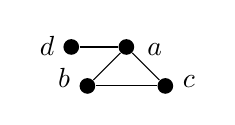
\begin{tikzpicture}[node distance=7mm,every node/.style={fill,circle,inner sep=2pt}]
\node (a) [label={[text height=1.5ex,yshift=0.0cm,xshift=0.05cm]left:$d$}] {};
\node (b) [right of=a,label={[text height=1.5ex]right:$a$}] {};
\node (c) [below left of=b,label={[text height=1.5ex,yshift=0.09cm,xshift=0.05cm]left:$b$}] {};
\node (d) [below right of=b,label={[text height=1.5ex,yshift=0.09cm,xshift=-0.05cm]right:$c$}] {};
%
\draw (a) to (b);
%
\draw (b) to (c);
\draw (b) to (d);
\draw (c) to (d);
%
\end{tikzpicture}\hspace{1em}%
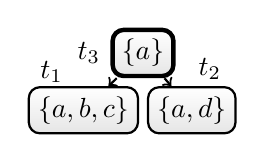
\begin{tikzpicture}[node distance=0.5mm]
%
\tikzset{every path/.style=thick}

\node (leaf1) [tdnode,label={[yshift=-0.25em,xshift=0.5em]above left:$t_1$}] {$\{a,b,c\}$};
\node (leaf2) [tdnode,label={[xshift=-1.0em, yshift=-0.15em]above right:$t_2$}, right = 0.1cm of leaf1]  {$\{a,d\}$};
\coordinate (middle) at ($ (leaf1.north east)!.5!(leaf2.north west) $);
\node (join) [tdnode,ultra thick,label={[]left:$t_3$}, above  = 1mm of middle] {$\{a\}$};

\coordinate (top) at ($ (join.north east)+(3.5em,0) $);
\coordinate (bot) at ($ (top)+(0,-4em) $);

%
\draw [->] (join) to (leaf1);
\draw [->] (join) to (leaf2);
\end{tikzpicture}%
\caption{Primal graph~$P_F$ of~$F$ from Example~\ref{ex:running0}
  (left) with a TD~${\cal T}$ of graph~$P_F$
  (right).}%
\label{fig:graph-td}%
\end{figure}

\begin{figure}[t]
\centering
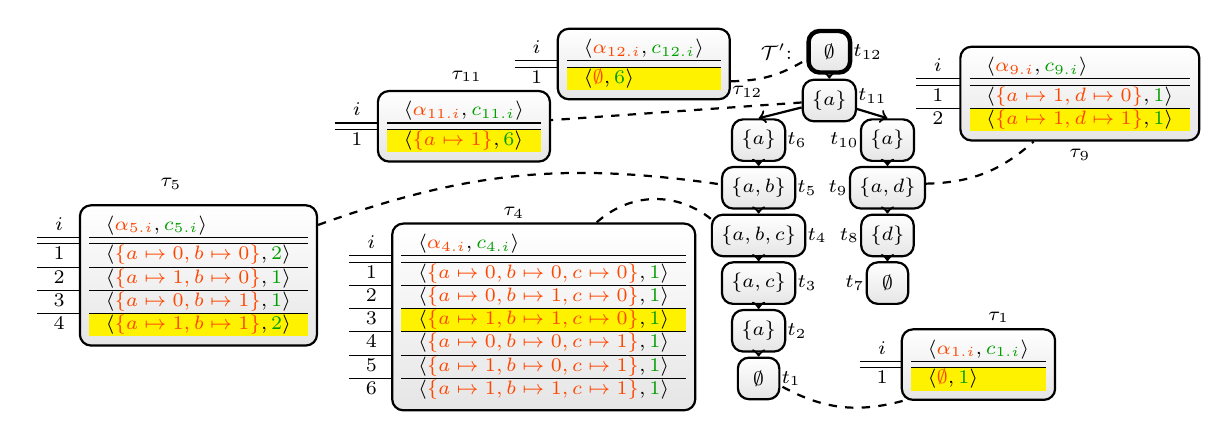
\begin{tikzpicture}[node distance=0.5mm]
%
\tikzset{every path/.style=thick}

%
\node (l1) [stdnode,label={[tdlabel, xshift=0em,yshift=+0em]right:${t_1}$}]{$\emptyset$};
\node (i1) [stdnode, above=of l1, label={[tdlabel, xshift=0em,yshift=+0em]right:${t_2}$}]{$\{a\}$};
\node (i12) [stdnode, above=of i1, label={[tdlabel, xshift=0em,yshift=+0em]right:${t_3}$}]{$\{a,c\}$};
\node (i13) [stdnode, above=of i12, label={[tdlabel, xshift=0em,yshift=+0em]right:${t_4}$}]{$\{a,b,c\}$};
\node (r1) [stdnode, above=of i13, label={[tdlabel, xshift=0em,yshift=+0em]right:${t_5}$}]{$\{a,b\}$};
\node (r12) [stdnode, above=of r1, label={[tdlabel, xshift=0em,yshift=+0em]right:${t_6}$}]{$\{a\}$};
\node (l2) [stdnode, right=2.5em of i12, label={[tdlabel, xshift=0em,yshift=+0em]left:${t_7}$}]{$\emptyset$};
\node (i2) [stdnode, above=of l2, label={[tdlabel, xshift=0em,yshift=+0em]left:${t_8}$}]{$\{d\}$};
\node (i22) [stdnode, above=of i2, label={[tdlabel, xshift=0em,yshift=+0em]left:${t_9}$}]{$\{a,d\}$};
\node (r2) [stdnode, above=of i22, label={[tdlabel, xshift=0em,yshift=+0em]left:${t_{10}}$}]{$\{a\}$};
\node (j) [stdnode, above left=of r2, yshift=-0.25em, label={[tdlabel, xshift=0em,yshift=+0.15em]right:${t_{11}}$}]{$\{a\}$};
\node (rt) [stdnode,ultra thick, above=of j, label={[tdlabel, xshift=0em,yshift=+0em]right:${t_{12}}$}]{$\emptyset$};
\node (label) [font=\scriptsize,left=of rt]{${\cal T}'$:};
%
\node (leaf1) [stdnode, left=1.25em of i1, yshift=0.5em, label={[tdlabel, xshift=2.75em,yshift=+.1em]above left:$\tab{4}$}]{%
	\begin{tabular}{l}%
		\multicolumn{1}{l}{$\langle \tuplecolor{\inputPredColor}{\alpha_{4.i}}, \tuplecolor{\statePredColor}{c_{4.i}} \rangle$}\\
		%
		\hline\hline
		$\langle \tuplecolor{\inputPredColor}{\{a\mapsto 0, b\mapsto 0, c\mapsto 0\}}, \tuplecolor{\statePredColor}{1}\rangle$\\\hline
		$\langle \tuplecolor{\inputPredColor}{\{a\mapsto 0, b\mapsto 1, c\mapsto 0\}}, \tuplecolor{\statePredColor}{1}\rangle$\\\hline
		\rowcolor{yellow}$\langle\tuplecolor{\inputPredColor}{\{a\mapsto 1,b\mapsto 1, c\mapsto 0\}}, \tuplecolor{\statePredColor}{1}\rangle$\\\hline
		$\langle \tuplecolor{\inputPredColor}{\{a\mapsto 0, b\mapsto 0, c\mapsto 1\}}, \tuplecolor{\statePredColor}{1}\rangle$\\\hline
		$\langle\tuplecolor{\inputPredColor}{\{a\mapsto 1,b\mapsto 0,c\mapsto 1\}}, \tuplecolor{\statePredColor}{1}\rangle$\\\hline
		$\langle\tuplecolor{\inputPredColor}{\{a\mapsto 1,b\mapsto 1,c\mapsto 1\}}, \tuplecolor{\statePredColor}{1}\rangle$\\
	\end{tabular}%
};
\node (leaf1b) [stdnodenum,left=of leaf1,xshift=0.6em,yshift=0pt]{%
	\begin{tabular}{c}%
		\multirow{1}{*}{$i$}\\ %
		%
		\hline\hline
		$1$ \\\hline
		$2$ \\\hline
		$3$ \\\hline
		$4$ \\\hline
		$5$ \\\hline
		$6$
	\end{tabular}%
};
\node (leaf0x) [stdnode, left=0.75em of leaf1b, yshift=1.5em, label={[tdlabel, xshift=2em,yshift=+.5em]above left:$\tab{5}$}]{%
	\begin{tabular}{l}%
		\multicolumn{1}{l}{$\langle \tuplecolor{\inputPredColor}{\alpha_{5.i}}, \tuplecolor{\statePredColor}{c_{5.i}} \rangle$}\\
		%
		\hline\hline
		$\langle \tuplecolor{\inputPredColor}{\{a\mapsto 0, b\mapsto 0\}}, \tuplecolor{\statePredColor}{2}\rangle$\\\hline
		%
		$\langle\tuplecolor{\inputPredColor}{\{a\mapsto 1, b\mapsto 0\}}, \tuplecolor{\statePredColor}{1}\rangle$\\\hline
		$\langle\tuplecolor{\inputPredColor}{\{a\mapsto 0,b\mapsto 1\}}, \tuplecolor{\statePredColor}{1}\rangle$\\\hline
		\rowcolor{yellow}$\langle\tuplecolor{\inputPredColor}{\{a\mapsto 1,b\mapsto 1\}}, \tuplecolor{\statePredColor}{2}\rangle$\\
	\end{tabular}%
};
\node (leaf0b) [stdnodenum,left=of leaf0x,xshift=0.6em,yshift=0pt]{%
	\begin{tabular}{c}%
		\multirow{1}{*}{$i$}\\ %
		%
		\hline\hline
		$1$ \\\hline
		$2$ \\\hline
		$3$ \\\hline
		$4$ %
	\end{tabular}%
};
\node (leaf2b) [stdnodenum,right=2.5em of j,xshift=-0.75em,yshift=+0.25em]  {%
	\begin{tabular}{c}%
		\multirow{1}{*}{$i$}\\ %
		%
		\hline\hline
		$1$\\\hline
		$2$\\%\hline
		%
	\end{tabular}%
};
\node (leaf2) [stdnode,right=-0.4em of leaf2b, label={[tdlabel, xshift=0em,yshift=-0.25em]below:$\tab{9}$}]  {%
	\begin{tabular}{l}%
		\multirow{1}{*}{$\langle \tuplecolor{\inputPredColor}{\alpha_{9.i}}, \tuplecolor{\statePredColor}{c_{9.i}} \rangle$}\\ %
		%
		\hline\hline
		$\langle \tuplecolor{\inputPredColor}{\{a\mapsto 1, d\mapsto 0\}}, \tuplecolor{\statePredColor}{1}\rangle$\\\hline
		%
		\rowcolor{yellow}$\langle \tuplecolor{\inputPredColor}{\{a\mapsto 1,d\mapsto 1\}}, \tuplecolor{\statePredColor}{1}\rangle$\\
	\end{tabular}%
};
\coordinate (middle) at ($ (leaf1.north east)!.5!(leaf2.north west) $);
\node (join) [stdnode,left=6.5em of r12, yshift=0.5em, label={[tdlabel, xshift=2em,yshift=+0.25em]above left:$\tab{{11}}$}] {%
	\begin{tabular}{l}%
		\multirow{1}{*}{$\langle \tuplecolor{\inputPredColor}{\alpha_{11.i}}, \tuplecolor{\statePredColor}{c_{11.i}} \rangle$}\\
		\hline\hline
		%
		%
		%
		\rowcolor{yellow}$\langle \tuplecolor{\inputPredColor}{\{a\mapsto 1\}}, \tuplecolor{\statePredColor}{6} \rangle$\\
	\end{tabular}%
};
\node (joinb) [stdnodenum,left=-0.45em of join] {%
	\begin{tabular}{c}
		\multirow{1}{*}{$i$}\\
		\hline\hline
		%
		%
		%
		$1$\\
	\end{tabular}%
};
\node (rtx) [stdnode,left=0.0em of r12, yshift=2.75em, label={[tdlabel, xshift=0em,yshift=-1em]right:$\tab{{12}}$}] {%
	\begin{tabular}{l}%
		\multirow{1}{*}{$\langle \tuplecolor{\inputPredColor}{\alpha_{12.i}}, \tuplecolor{\statePredColor}{c_{12.i}} \rangle$}\\
		\hline\hline
		%
		%
		%
		\rowcolor{yellow}$\langle \tuplecolor{\inputPredColor}{\emptyset}, \tuplecolor{\statePredColor}{6} \rangle$\\
	\end{tabular}%
};
\node (rtb) [stdnodenum,left=-0.45em of rtx] {%
	\begin{tabular}{c}
		\multirow{1}{*}{$i$}\\
		\hline\hline
		%
		%
		%
		$1$\\
	\end{tabular}%
};
\node (leaf0n) [stdnodenum,yshift=0.5em, right=2.5em of l1] {%
	\begin{tabular}{c}%
		\multirow{1}{*}{$i$}\\ %
		%
		\hline\hline
		$1$
	\end{tabular}%
};
%
\node (leaf0) [stdnode,right=-0.5em of leaf0n, label={[tdlabel, xshift=-1em,yshift=0.15em]above right:$\tab{1}$}] {%
	\begin{tabular}{l}%
		\multicolumn{1}{l}{$\langle \tuplecolor{\inputPredColor}{\alpha_{1.i}}, \tuplecolor{\statePredColor}{c_{1.i}} \rangle$}\\
		%
		\hline\hline
		\rowcolor{yellow}$\langle \tuplecolor{\inputPredColor}{\emptyset}, \tuplecolor{\statePredColor}{1} \rangle$
	\end{tabular}%
};
\coordinate (top) at ($ (leaf2.north east)+(0.6em,-0.5em) $);
\coordinate (bot) at ($ (top)+(0,-12.9em) $);

\draw [<-] (j) to (rt);
\draw [->] (j) to ($ (r12.north)$);
%
%
\draw [->] (j) to ($ (r2.north)$);
\draw [->](r2) to (i22);
\draw [<-](i2) to (i22);
\draw [<-](l2) to (i2);
\draw [<-](l1) to (i1);
\draw [->](i12) to (i1);
\draw [->](i13) to (i12);
\draw [->](r1) to (i13);
\draw [->](r12) to (r1);

\draw [dashed, bend left=0] (j) to (join);
\draw [dashed, bend right=15] (rtx) to (rt);
\draw [dashed, bend right=20] (i22) to (leaf2);
\draw [dashed, bend right=40] (i13) to (leaf1);
%
\draw [dashed, bend left=22] (leaf0) to (l1);
\draw [dashed, bend left=14] (leaf0x) to (r1);
%
%
\end{tikzpicture}
\caption{Selected tables obtained by dynamic programming of instance~$F$ in Example~\ref{ex:running0} using algorithm~${\algo{K}}$ on tree decomposition~${\cal T}'$.}
\label{fig:running1}
\end{figure}




\subsection{Detailed Results}

\begin{table}
  \resizebox{\columnwidth}{!}{%
    \begin{tabular}{{l|rr|rr||rrr||rrr||rrrrr|rrrr}}
      \toprule
      set & N & pre & vMdn& cMdn & t[s] Mdn & t[s] Max & to & t[s] Mdn pre & t[s] Max pre & to & Mdn & 50\% & 80\% & 90\% & 95\% & min & max & mdn & mean \\
      \midrule
      \# Proj. & 308 & w/o pre & 68056 & 74016 & 65.39 & 1800.0 & 6 & 0.0 & 0.0 & 0 & 302 & 328 & 1084 & 1872 & ??? & 0 & 0 & 0.0 & 0 \\
      &  & pmc, B+E & 35762 & 49417 & 29.4 & 1800.0 & 6 & 900.0 & 900.0 & 192 & 179 & 192 & 922 & 1609 & 2225 & -72 & 755 & 0 & 46.33 \\
      &  & pmc & 35762 & 43769 & 28.27 & 1800.0 & 6 & 211.81 & 900.0 & 103 & 178 & 200 & 988 & 1888 & 2662 & -1839 & 547 & 31 & 10.59 \\
      &  & B+E & 35762 & 49601 & 29.08 & 1800.0 & 6 & 900.0 & 900.0 & 189 & 178 & 183 & 949 & 1609 & 2225 & 0 & 633 & 0.0 & 48.05 \\
      \# Weig. & 1080 & w/o pre & 200 & 518 & 0.05 & 1.31 & 0 & 0.0 & 0.0 & 0 & 28 & 28 & 40 & 43 & 48 & 0 & 0 & 0.0 & 0 \\
      &  & pmc, B+E & 200 & 250 & 0.02 & 0.46 & 0 & 0.02 & 35.84 & 0 & 3 & 3 & 9 & 12 & 15 & 2 & 79 & 23.0 & 25.6 \\
      &  & pmc & 200 & 123 & 0.02 & 0.58 & 0 & 0.01 & 13.91 & 0 & 3 & 3 & 9 & 13 & 16 & 1 & 81 & 23.0 & 25.11 \\
      &  & B+E & 200 & 128 & 0.02 & 0.48 & 0 & 0.01 & 33.36 & 0 & 3 & 3 & 9 & 13 & 16 & 2 & 80 & 24 & 26.19 \\
      \# Basic & 92 & w/o pre & 604 & 1680 & 0.12 & 9.31 & 0 & 0.0 & 0.0 & 0 & 26 & 26 & 63 & 85 & 110 & 0 & 0 & 0.0 & 0 \\
      &  & pmc, B+E & 604 & 615 & 0.03 & 1.75 & 0 & 0.07 & 35.67 & 0 & 9 & 9 & 18 & 30 & 40 & -2 & 351 & 21.5 & 37.66 \\
      &  & pmc & 604 & 794 & 0.04 & 8.58 & 0 & 0.05 & 24.05 & 0 & 14 & 15 & 44 & 61 & 88 & 0 & 324 & 9.0 & 24.87 \\
      &  & B+E & 604 & 701 & 0.03 & 1.51 & 0 & 0.05 & 45.52 & 0 & 9 & 9 & 18 & 27 & 35 & -2 & 349 & 22.0 & 37.3 \\
      \# Mixed & 14 & w/o pre & 1286 & 11370 & 1.36 & 16.01 & 0 & 0.0 & 0.0 & 0 & 57 & 63 & 399 & 442 & 540 & 0 & 0 & 0.0 & 0 \\
      &  & pmc, B+E & 1286 & 3196 & 0.23 & 4.12 & 0 & 0.74 & 3.5 & 0 & 41 & 50 & 112 & 133 & 158 & 0 & 428 & 32.5 & 123.71 \\
      &  & pmc & 1286 & 3760 & 0.38 & 4.25 & 0 & 0.41 & 1.58 & 0 & 41 & 50 & 137 & 164 & 183 & 0 & 403 & 34.0 & 115.86 \\
      &  & B+E & 1286 & 3278 & 0.27 & 4.28 & 0 & 0.48 & 2.52 & 0 & 52 & 54 & 117 & 141 & 190 & 0 & 423 & 8.0 & 112 \\
      \bottomrule
    \end{tabular}
  }
  \caption{Detailed results on upper bounds of the primal treewidth for the considered~\cSAT benchmark sets before and after preprocessing.}
  \label{tab:det}
\end{table}

Table~\ref{tab:det} contains detailed results grouped by benchmark set
and shows significant improvements for all benchmark sets.
%
Even when considering the hard set~\set{\#Proj}, we observe that we
could significantly reduce the treewidth upper bounds and could
decompose more than~95\% of those instances.  Note that we could
decompose almost all the instances within 1800 seconds, only 6
instances of set~\set{\#Proj} timed out during decomposition (both
before and after preprocessing). %
%
%
%
%
%
%
%
%
%
%
%
%
%
%
%
%
%
%
%



\end{document}

%





%
%
%
%
%
%
%
%
%
%
%
%
%
%
%
%
%
%
%
%
%
%
%
%
%
%
%
%
%
%
%
%
%
%
%
%
%
%
%
%
%
%
%
%


%
%
%
%
%
%
%
%
%
%
%
%
%
%
%
%
%
%
%
%
%
%
%
%
%
%
%
%
%
%
%
%
%
%
%
%
%
%
%
%
%
%
%
%
%
%
%
%
%
%
%
%
%
%
%
%
%
%
%
%
%
%
%
%
%
%
%
%
%
%
%

%
Intuitively, algorithm~\algo{K} stores in table~$\tab{t}$ only
assignments restricted to bag~$\chi_t$, %
%
and its counters.
%
%
%
%
The stored counters allow to reconstruct the number of
%
%
satisfying assignments of the \emph{formula~$F_{\leq t}$ below~$t$},
which consists of~$F_{t'}$ for each descendant~$t'$ of~$t$ in~$T$.
%
In the end, we can simply read the solution from the table at the root.


%
%
%
%
%
%
%
%
%
%
%
%
%
%
%
%
%


%

%
%
%
%
%

%

%
%

%


%
%
%
%
%
%
%
%
%



%

%
%
%
%
%
%
%


%
%

%
%
%
%

%
%
%
%
